% Harus dimuat terlebih dahulu, digunakan agar file PDF memiliki format karakter yang benar.
% Untuk informasi lebih lanjut, lihat https://ctan.org/pkg/cmap.
\RequirePackage{cmap}

% Format dokumen sebagai paper konferensi menggunakan aturan IEEEtran terbaru (v1.8b).
% Untuk informasi lebih lanjut, lihat http://www.michaelshell.org/tex/ieeetran/.
\documentclass[a4paper, conference]{IEEEtran}

% Format encoding font dan input menjadi 8-bit UTF-8.
\usepackage[T1]{fontenc}
\usepackage[utf8]{inputenc}
\usepackage{amsmath}

% Digunakan untuk mengatur margin dokumen.
\usepackage{textcomp}

% Format bahasa menjadi bahasa indonesia dan inggris.
\usepackage[indonesian]{babel}

% Digunakan untuk tujuan demonstrasi.
\usepackage{mwe}

% Digunakan untuk menampilkan font dengan style yang lebih baik.
\usepackage[zerostyle=b,scaled=.75]{newtxtt}

% Digunakan untuk menampilkan tabel dengan style yang lebih baik.
\usepackage{booktabs}
\usepackage[table,xcdraw]{xcolor}
% Digunakan untuk menampilkan gambar pada dokumen.
\usepackage{graphicx}

% Digunakan untuk menampilkan potongan kode.
\usepackage{listings}
\lstset{
  basicstyle=\ttfamily,
  columns=fixed,
  basewidth=.5em,
  xleftmargin=0.5cm,
  captionpos=b
}

\usepackage{tabularx}
\usepackage{float}
\usepackage{wrapfig}
% Digunakan agar backticks (`) dapat dirender pada PDF.
% Untuk informasi lebih lanjut, lihat https://tex.stackexchange.com/a/341057/9075.
\usepackage{upquote}

% Digunakan untuk menyeimbangkan bagian akhir dokumen dengan dua kolom.
\usepackage{balance}

% Kapitalisasi caption tabel
\usepackage{caption}
\captionsetup[table]{
    justification=centering, % Memusatkan caption
    labelsep=newline, % Memisahkan label "TABLE 1" dengan judul dengan baris baru
    textfont={sc}, % Membuat teks menjadi kapital
    labelfont={sc} % Membuat teks menjadi kapital
}


% Digunakan untuk menampilkan pustaka.
\usepackage[square,comma,numbers,sort&compress]{natbib}

% Mengubah format ukuran teks pada natbib.
\renewcommand{\bibfont}{\normalfont\footnotesize}

% Jika melebihi 3 penulis dapat dilakukan linebreakend 
\makeatletter
\newcommand{\linebreakand}{%
  \end{@IEEEauthorhalign}
  \hfill\mbox{}\par
  \mbox{}\hfill\begin{@IEEEauthorhalign}
}
\makeatother

% Menambah nama penulis ketika menggunakan perintah \citet.
% Untuk informasi lebih lanjut, lihat https://tex.stackexchange.com/a/76075/9075.
\usepackage{etoolbox}
\makeatletter
\patchcmd{\NAT@test}{\else \NAT@nm}{\else \NAT@hyper@{\NAT@nm}}{}{}
\makeatother

% Digunakan untuk melakukan linewrap pada pustaka dengan url yang panjang
% jika terdapat hyphens
\usepackage[hyphens]{url}

% Digunakan untuk menambah hyperlink pada referensi.
\usepackage{hyperref}

% Menonaktifkan warna dan bookmark pada hyperref.
\hypersetup{hidelinks,
  colorlinks=true,
  allcolors=black,
  pdfstartview=Fit,
  breaklinks=true
}

% Digunakan untuk membenarkan hyperref pada gambar.
\usepackage[all]{hypcap}

% Digunakan untuk menampilkan beberapa gambar
\usepackage[caption=false,font=footnotesize]{subfig}

\usepackage{stfloats}
% nama
\newcommand{\name}{I Putu Krisna Erlangga}
\newcommand{\authorname}{Erlangga, I Putu Krisna}
\newcommand{\nickname}{Krisna}
\newcommand{\advisor}{Dr. Eko Mulyanto Yuniarno, S.T., M.T.}
\newcommand{\coadvisor}{Dr. Diah Puspito Wulandari, S.T., M.Sc.}

% identitas
\newcommand{\nrp}{5024 20 1055}
\newcommand{\advisornip}{19740907 200212 1 001}
\newcommand{\coadvisornip}{19680601 199512 1 009}
\newcommand{\email}{5024201055@student.its.ac.id}

\newcommand{\advisoremail}{ekomulyanto@ee.its.ac.id}
\newcommand{\coadvisoremail}{diah@te.its.ac.id}

% judul
\newcommand{\tatitle}{PENERJEMAH BAHASA ISYARAT INDONESIA (BISINDO) KE MEDIA SUARA MENGGUNAKAN \emph{LONG SHORT-TERM MEMORY} (LSTM) BERBASIS INTEL \emph{NEXT UNIT COMPUTING} (NUC)}
\newcommand{\engtatitle}{\emph{TRANSLATOR OF INDONESIAN SIGN LANGUAGE (BISINDO) TO VOICE MEDIA USING LONG SHORT-TERM MEMORY (LSTM) BASED ON INTEL NEXT UNIT COMPUTING (NUC)}}

% tempat
\newcommand{\place}{Surabaya}

% jurusan
\newcommand{\studyprogram}{Teknik Komputer}
\newcommand{\engstudyprogram}{Computer Engineering}

% fakultas
\newcommand{\faculty}{Teknologi Elektro dan Informatika Cerdas}
\newcommand{\engfaculty}{Intelligence Electrical and Informatics Technology}

% singkatan fakultas
\newcommand{\facultyshort}{FTEIC}
\newcommand{\engfacultyshort}{ELECTICS}

% departemen
\newcommand{\department}{Teknik Komputer}
\newcommand{\engdepartment}{Computer Engineering}

\input{pustaka/tanda-hubung.tex}

\begin{document}

\input{deskripsi/judul.tex}
% Mengubah keterangan `Abstract` ke bahasa indonesia.
% Hapus bagian ini untuk mengembalikan ke format awal.
\renewcommand\abstractname{Abstrak}

\begin{abstract}

  % Ubah paragraf berikut sesuai dengan abstrak dari penelitian.
Tunarungu menggunakan bahasa isyarat sebagai bahasa komunikasi utama. Menurut GERKATIN terdapat setidaknya 2,9 juta orang penyandang tunarungu. Hal ini tidak diikuti dengan pengetahuan masyarakat umum mengenai bahasa isyarat yang berdampak pada sulitnya komunikasi tunarungu dengan masyarakat sekitar sehingga adanya keterbatasan dalam peningkatan kualitas hidup mereka. Sistem penerjemah saat ini masih terbatas dalam menerjemahkan dalam bentuk kata saja dan belum adanya upaya dalam membuat sistem yang bersifat inklusif. Pada penelitian ini telah dikembangkan sistem penerjemah BISINDO menggunakan arsitektur LSTM. Sistem telah diimplementasikan pada Intel NUC dengan kemampuan dalam menerjemahkan gerakan isyarat secara \emph{real time}. Pengguna dapat membentuk kalimat - kalimat yang umum digunakan sehari - hari dan mengkonversinya ke media suara dengan bantuan gerakan isyarat kontrol. Berdasarkan pengujian yang telah dilakukan, didapat bahwa sistem dapat beradaptasi dengan adanya perbedaan intensitas cahaya, jarak, serta subjek yang berbeda dengan penulis dengan akurasi tertinggi mencapai 100\%. Sistem ini dapat menjadi solusi dalam mengatasi hambatan komunikasi antara tunarungu dengan khalayak umum.

\end{abstract}

% Mengubah keterangan `Index terms` ke bahasa indonesia.
% Hapus bagian ini untuk mengembalikan ke format awal.
\renewcommand\IEEEkeywordsname{Kata kunci}

\begin{IEEEkeywords}

  % Ubah kata-kata berikut sesuai dengan kata kunci dari penelitian.
  Tunarungu, BISINDO, LSTM, Intel NUC

\end{IEEEkeywords}


% Ubah bagian berikut sesuai dengan konten-konten yang akan dimasukkan pada dokumen
% Ubah judul dan label berikut sesuai dengan yang diinginkan.
\section{Pendahuluan}
\label{sec:pendahuluan}

% Ubah paragraf-paragraf pada bagian ini sesuai dengan yang diinginkan.

Bahasa isyarat merupakan bahasa yang mengutamakan komunikasi manual dengan mengkombinasikan bentuk tangan, orientasi gerak tangan, lengan, bibir, ataupun ekspresi mimik wajah untuk mengungkapkan sesuatu. Tunarungu merupakan kondisi ketidakmampuan seorang dalam menangkap rangsangan secara auditori melalui indra pendengarannya \cite{maulida2017}. Penyandang tunarungu menggunakan bahasa isyarat dalam berkomunikasi, baik kepada sesama penyandang tunarungu ataupun masyarakat sekitar. Di Indonesia, bahasa isyarat Indonesia (BISINDO) merupakan bahasa isyarat yang lebih umum digunakan dalam kehidupan sehari - hari. GERKATIN (Gerakan untuk Kesejahteraan Tunarungu Indonesia) mencatat terdapat setidaknya 2,9 juta orang atau sekitar 1,25\% dari total populasi penduduk Indonesia yang merupakan masyarakat penyandang tunarungu \cite{evitasari2015}. Namun, kurangnya pemahaman masyarakat tentang bahasa isyarat menyebabkan penyandang tunarungu kesulitan berkomunikasi, sehingga membatasi kualitas hidup mereka. Perkembangan teknologi saat ini telah menghasilkan berbagai inovasi yang membantu manusia dalam kehidupan sehari-hari, termasuk \emph{deep learning}.Salah satu arsitekturnya \emph{deep learning}, \emph{Long Short-Term Memory} (LSTM), dapat menyimpan informasi masa lampau dan mempelajari berbentuk data sekuensial. LSTM ideal untuk menerjemahkan bahasa isyarat karena memiliki pola sekuensial \cite{sadli2020}. Penelitian sebelumnya oleh Putri et al. berhasil mengembangkan deteksi real-time BISINDO dengan akurasi 65\% pada 30 kelas kata \cite{putri2022}. Sedangkan penelitian oleh Suhartijo dan Aljabar mencapai 86\% akurasi pada 10 kelas menggunakan LSTM \cite{aljabar2020}. Selain itu, perkembangan teknologi juga melahirkan perangkat bernama \emph{mini computer} yangmemiliki fungsi seperti komputer biasa, namun dalam ukuran lebih kecil dengan keunggulan ringan, ringkas, efisiensi energi, dan harga terjangkau. Pada tahun 2013, Intel mengeluarkan mini PC bernama Intel Next Unit Computing (NUC), yang menjadi solusi perangkat dengan kemampuan komputasi dan mobilitas tinggi \cite{minny2023}. Oleh karena itu, dibutuhkan suatu sistem penerjemah BISINDO ke media suara sebagai salah satu solusi dalam mengatasi masalah komunikasi antar penyandang tuna rungu dengan masyarakat umum dan mendukung GERKATIN dalam menggantikan bahasa isyarat nasional. Sistem penerjemah saat ini masih diimplementasikan secara pada laptop saja sehingga Intel \emph{Next Unit Computing} menjadi perangkat yang akan diimplementasikan sistem penerjemah bahasa isyarat sebagai upaya awal dalam menciptakan sistem penerjemah yang dapat dijangkau oleh masyarakat luas.
% Ubah judul dan label berikut sesuai dengan yang diinginkan.
\section{Tinjauan Pustaka}
\label{sec:tinjauanpustaka}

\subsection{Penelitian Terdahulu}
\label{subsec:penelitianterdahulu}

Penelitian yang dilakukan oleh Andi Aljabar dan Suhartijo berhasil menerjemahkan bahasa isyarat Indonesia dengan arsitektur Convolutional Neural Network (CNN), Long Short-Term Memory (LSTM), dan kombinasi keduanya. Pengujian dengan 10 kelas kosakata BISINDO menunjukkan akurasi rata-rata 73\% pada CNN, 81\% pada LSTM, dan 90\% pada gabungan CNN-LSTM \cite{aljabar2020}. Penelitian oleh Husna Moetia Putri, Fadlisyah, dan Wahyu Fuadi mendeteksi bahasa isyarat secara real-time menggunakan LSTM dan MediaPipe Holistic. Evaluasi pada 10 kosakata BISINDO mencapai akurasi 92\% dan pada 30 kosakata akurasi mencapai 65\% \cite{putri2022}. Siti Nur, Aghisna Nur Assyifa, dan Habilah Nurjannah mengembangkan aplikasi penerjemah BISINDO menggunakan LSTM dengan akurasi 75\% pada 500 data, meningkat menjadi 85\% pada 1000 dan 1500 data. Aplikasi ini memiliki fitur menambah kosakata dan menyimpan data untuk menghasilkan output kosakata isyarat yang sesuai \cite{nur2023}.

\subsection{Bahasa Isyarat Indonesia (BISINDO)}
\label{subsec:tunarungu}

Tunarungu adalah istilah untuk seseorang yang kehilangan atau tidak mampu menangkap rangsangan auditori melalui indra pendengarannya \cite{mursita2015}. Berdasarkan kelahiran, tunarungu dapat dibagi menjadi dua, yaitu \emph{congenitally deaf} (sejak lahir) dan \emph{adventitiously deaf} (karena penyakit atau peristiwa traumatis). Tunarungu juga diklasifikasikan berdasarkan tingkat kemampuan pendengaran dalam \emph{decibel} (dB), dari ringan hingga total \cite{winarsih2007}. Di Indonesia, terdapat setidaknya 2,9 juta atau 1,25\% penduduk yang merupakan penyandang tunarungu \cite{evitasari2015}. 
Penyandang tunarungu menggunakan bahasa isyarat dalam berkomunikasi. Bahasa isyarat adalah bahas yang diungkapkan dengan kombinasi antara bentuk tangan, orientasi dan gerak tangan, lengan tubuh, serta ekspresi wajah \cite{mursita2015}. Terdapat dua bahasa isyarat yang berkembang di Indonesia, yaitu Sistem Bahasa Isyarat Indonesia (SIBI) dan Bahasa Isyarat Indonesia (BISINDO). SIBI menggunakan satu tangan, sedangkan BISINDO menggunakan dua tangan. BISINDO lebih umum digunakan karena tidak terikat struktur bahasa Indonesia dan berasal dari bahasa ibu tunarungu dan menyesuaikan pemahaman mereka tanpa menekankan struktur imbuhan bahasa Indonesia.

\subsection{Mediapipe}
\label{subsec:mediapipe}
MediaPipe adalah kerangka kerja (\emph{framework}) untuk membangun \emph{pipeline} inferensi pada data sensorik seperti audio dan video. Framework ini memungkinkan pembuatan pipeline yang terdiri dari komponen modular, seperti model inferensi, algoritma pemrosesan media, dan transformasi data. MediaPipe mengabstraksikan dan menghubungkan model-model persepsi individu ke dalam alur yang dapat dipertahankan, sehingga komponen dapat digunakan kembali. Konsep dasar MediaPipe mencakup kerangka kerja inferensi data sensorik, alat evaluasi kinerja, dan komponen pemrosesan yang dapat digunakan kembali. MediaPipe dirancang untuk mendukung pengembangan model \emph{machine learning} dan \emph{deep learning}, seperti deteksi objek dan pendeteksian gerakan bahasa isyarat \cite{lugaresi2019:}. Mediapipe Pose merupakan \emph{framework} yang dapat memprediksi total 33 lokasi \emph{landmark}, dengan diawali dari bagian hidung hingga diakhiri pada kaki bagian kanan. Mediapipe Hand merupakan \emph{framework} yang dapat memprediksi 21 lokasi \emph{landmark} yang meliputi keseluruhan tangan \cite{googleMediapipe}.


\subsection{\emph{Long Short Term-Memory} (LSTM)}
\label{subsec:lstm}

\begin{figure}[ht]
    \centering

    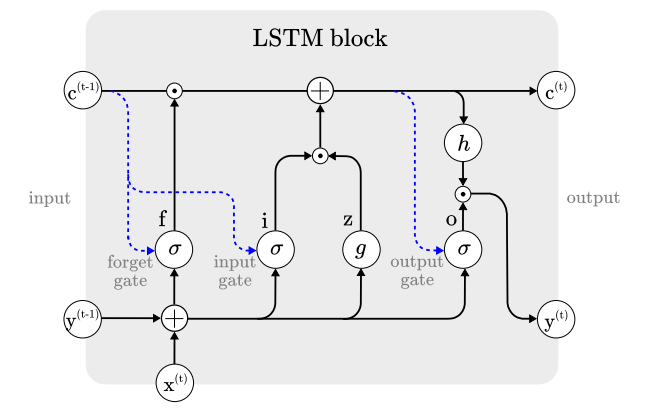
\includegraphics[scale=0.5]{gambar/bab2-lstm-model.png}
 
    \caption{Cara kerja arsitektur LSTM}
    \label{fig:longshortterm}
\end{figure}

\textit{Long Short-Term Memory} (LSTM) merupakan bentuk khusus dari neural network RNN atau \textit{Recurrent Neural Network} yang memiliki kemampuan \textit{feedback connection}. Kemampuan ini memungkinkan LSTM untuk dapat mengingat informasi untuk waktu yang lama sehingga dapat digunakan untuk menyelesaikan permasalahan yang memiliki sifat sekuensial atau berurutan. Keunggulan LSTM jika dibandingkan dengan RNN adalah LSTM memiliki kemampuan untuk mengingat informasi yang lebih baik dan efektif sehingga meminimalisir terjadinya kehilangan informasi yang umum terjadi pada pemrosesan informasi lama yang panjang pada penggunaan RNN \cite{xia2020}. LSTM sangat tepat digunakan untuk melakukan klasifikasi bahasa isyarat yang bersifat sekuensial. Pada gambar \ref{fig:longshortterm}, \textit{Long Short-Term Memory} tersusun atas beberapa layer yang meliputi \textit{block input}, \textit{input gate}, \textit{forget gate}, \textit{cell}, \textit{output gate}, dan \textit{block output} yang dapat dirumuskan secara berurutan sebagai berikut:

\begin{equation}
    \label{eq:blockinputLSTM}
    x^{(t)} = g(W_z x^{(t)} + R_z y^{(t-1)} + b_z)
  \end{equation}

  \begin{equation}
    \label{eq:inputgateLSTM}
    i^{(t)} = \sigma(W_i x^{(t)} + R_i y^{(t-1)}+ p_i \odot c^{(t-1)} + b_i)
\end{equation}

\begin{equation}
    \label{eq:cellLSTM}
    c^{(t)} =  z^{(t)} \odot  i^{(t)} + z^{(t-1)} \odot  f^{(t)}
\end{equation}

\begin{equation}
    \label{eq:outputgateLSTM}
    o^{(t)} = \sigma(W_o x^{(t)} + R_o y^{(t-1)}+ p_o \odot c^{(t)} + b_o)
\end{equation}

\subsection{Intel \emph{Next Unit Computing} (NUC)}
\label{subsec:intelNUC}

Intel \emph{Next Unit Computing} (NUC) merupakan komputer \emph{barebone} dengan ukuran kecil yang dirancang oleh Intel. Intel NUC merupakan perangkat yang berfokus dalam menyediakan komputasi kuat dalam ukuran yang praktis dan dapat melayani berbagai kebutuhan pengguna, mulai dari bermain \emph{game}, bisnis, hingga menjalankan aplikasi kompleks. Intel NUC secara resmi memperkenalkan perangkat ini pada tahun 2012 dan dipasarkan secara umum pada awal tahun 2013 \cite{IntelNUC2020}. Adapun seri pertama dari Intel NUC memiliki CPU Sandy Bridger berbasis Celeron. Intel NUC telah berkembang hingga generasi ke-12 bernama Dragon Canyon yang dilengkapi dengan CPU Intel generasi ke-12 dan PCI Express Gen 5 \cite{Halfacree2013}.

% Beberapa penelitian lain pernah dilakukan seperti yang dirumuskan oleh \citet{newton1687} bahwa \lipsum[5]
% Hasil tersebut kemudian menjadi persamaan \ref{eq:hukumpertama}.

% % Contoh pembuatan persamaan ilmiah.
% \begin{equation}
%   \label{eq:hukumpertama}
%   \sum \mathbf{F} = 0\; \Leftrightarrow\; \frac{\mathrm{d} \mathbf{v} }{\mathrm{d}t} = 0.
% \end{equation}

% \lipsum[6-7]
% Ubah judul dan label berikut sesuai dengan yang diinginkan.
\section{Desain dan Implementasi}
\label{sec:desaindanimplementasi}

\begin{figure}[ht]
  \centering

  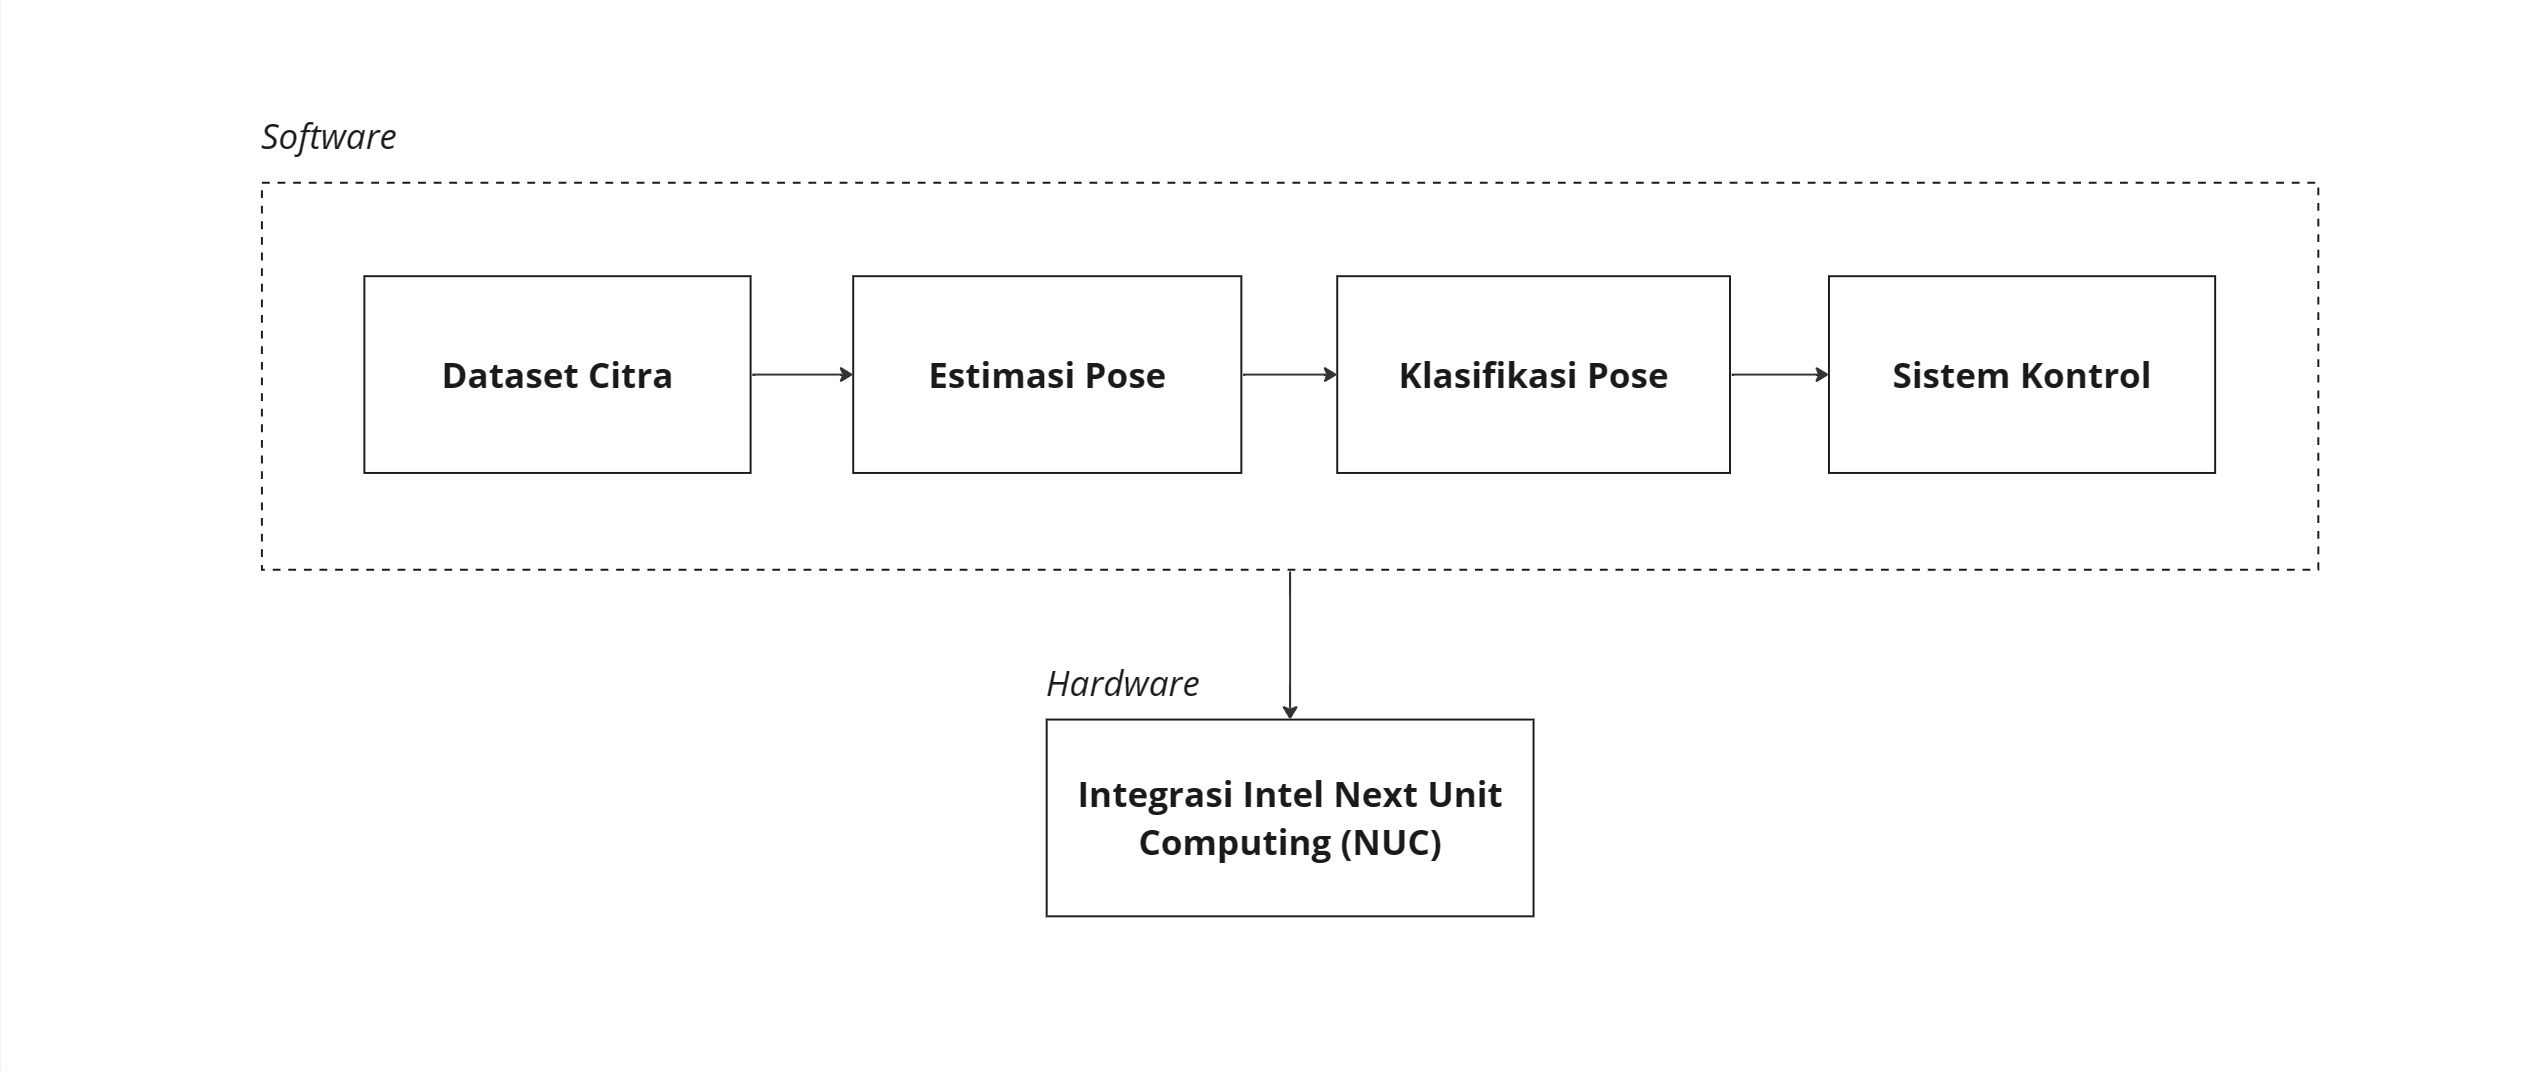
\includegraphics[scale=0.095]{gambar/bab3-block-diagram-nuc.jpg}

  \caption{Alur penelitian}
  \label{fig:blockdiagrammethod}
\end{figure}

\subsection{Dataset Citra}
\label{subsec:datasetcitra}

Dataset yang akan digunakan adalah kumpulan citra berukuran 640 pixel x 480 pixel. Data citra didapatkan dengan bantuan \emph{library} OpenCV untuk mengambil video dengan yang kemudian diekstrak menjadi 30 \emph{frame} untuk setiap data. Adapun digunakan 6 kosakata isyarat BISINDO dengan konteks kosakata umum dan 3 isyarat kontrol untuk memudahkan penggunaan sistem. 

\begin{table}[H]
  \caption{Kosakata BISINDO dan Kontrol}
  \label{tb:kosakataBISINDO}
  \centering
  \begin{tabular}{lll}
    \toprule
    \textbf{Kelas} & \textbf{Jumlah Data} & \textbf{Jumlah \emph{Frame}} \\
    \midrule
    Maaf                        & 30            & 30 \\
    Tolong                      & 30            & 30 \\
    Saya                        & 30            & 30 \\
    Nama                        & 30            & 30 \\
    Rumah                       & 30            & 30 \\
    Siapa                       & 30            & 30 \\
    \textit{Standby}                       & 30             & 30 \\
    \textit{Translate}                     & 30             & 30 \\
    \textit{Delete}                        & 30             & 30 \\
    \bottomrule
  \end{tabular}
\end{table}


\subsection{Estimasi Pose}
\label{subsec:estimasipose}

\begin{figure}[ht]
  \centering

  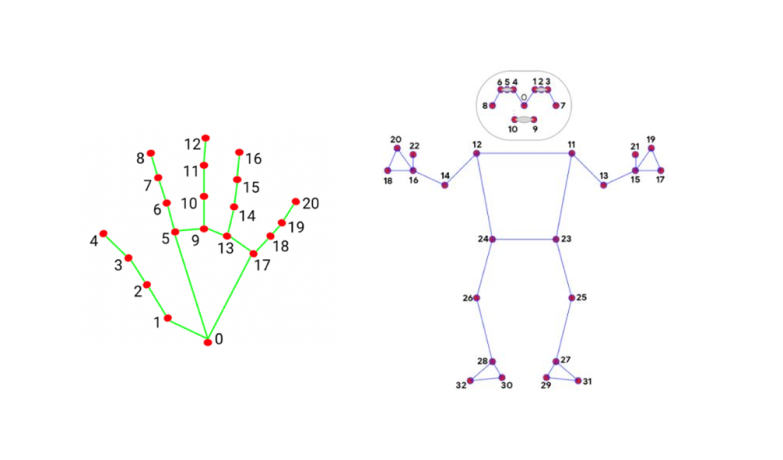
\includegraphics[scale=0.3]{gambar/bab3-pose-combine.png}

  \caption{Mediapipe Pose dan \emph{Hand}}
  \label{fig:estimasipose}
\end{figure}

Untuk setiap citra pada 30 data yang telah dilakukan estimasi pose dengan bantuan \textit{framework} MediaPipe. Dalam pembentukan isyarat BISINDO, bagian tubuh yang bergerak adalah bagian tangan dan lengan. Melalui MediaPipe hand akan dilakukan ekstraksi untuk 21 \textit{landmark} pada bagian tangan, sehingga total \textit{landmark} untuk tangan kanan dan kiri adalah 42 \textit{landmark}. Pada MediaPipe pose akan dilakukan ekstraksi pada bagian bahu sampai lengan sehingga \textit{landmark} yang akan digunakan hanya pada posisi 11 hingga 22 sehingga total \textit{landmark} untuk bagian tubuh adalah 12 \textit{landmark}. Untuk setiap \textit{landmark} yang didapatkan data koordinat x dan y. Data ini kemudian dilakukan normalisasi untuk menghasilkan model yang \textit{scale invariant} (adaptasi terhadap bentuk pengguna) dan \textit{position invariant} (adaptasi terhadap posisi pengguna). Adapun berikut adalah rumus normalisasi yang akan digunakan:

\begin{equation}
  \label{eq:shouderWidthNorm}
  w = \sqrt{(x_{ka} - x_{ki})^2 + (y_{ka} - y_{ki})^2}
\end{equation}

\begin{equation}
  \label{eq:shoulderMidpointNorm}
  x_m = \frac{x_{ka} + x_{ki}}{2} ; \\
   y_m = \frac{y_{ka} + y_{ki}}{2}
\end{equation}

\begin{equation}
  \label{eq:normalization}
  x'_i = \frac{x_i - x_m}{w} ;  \\
   y'_i = \frac{y_i - y_m}{w}
\end{equation}

\subsection{Klasifikasi Pose}
\label{subsec:klasifikasipose}

Model LSTM yang digunakan memiliki arsitektur sekuensial untuk menggabungkan serangkaian layer demi menghasilkan model penerjemah bahasa isyarat yang berperforma baik. Layer pertama adalah TimeDistributed dengan Dense layer berjumlah 128 unit, aktivasi 'tanh', dan input berbentuk (30, 108), di mana setiap frame diproses secara independen dengan konsistensi Dense layer untuk setiap frame. Layer kedua adalah LSTM pertama dengan 128 unit, return\_sequences=True, aktivasi 'tanh', dan input berbentuk (30, 108). Layer ketiga adalah Dropout layer dengan nilai 0,5 untuk mencegah weight yang terlalu tinggi. Layer keempat adalah LSTM kedua dengan 128 unit, return\_sequences=False, dan aktivasi 'tanh', diikuti Dropout layer dengan nilai 0,5. Untuk menyederhanakan kompleksitas data keluaran dari dua LSTM layer, digunakan Dense layer dengan 128 unit dan aktivasi 'relu', diikuti Dropout layer dengan nilai 0,2 untuk mencegah overfitting. Layer terakhir adalah Dense layer dengan aktivasi 'softmax' dan jumlah unit sesuai dengan jumlah kategori. Model ini dikompilasi menggunakan optimizer Adam dan categorical crossentropy sebagai fungsi loss, dengan metrik akurasi kategorikal untuk memantau performa selama pelatihan.

\subsection{Sistem Kontrol}
\label{subsec:sisitemkontrol}
Sistem kontrol adalah serangkaian proses yang akan mengatur bagaimana nantinya bahasa isyarat akan dideteksi, melakukan penanggulangan terhadap adanya kesalahan pendeteksian, menyatukan berbagai kata dalam bentuk kalimat, penghapusan kosakata, dan penerjemahan kalimat dalam bentuk suara. Penggunaan sistem kontrol ini diharapkan akan memudahkan pengguna dalam menggunakan sistem penerjemah. Sistem kontrol akan dibagi menjadi 2, yaitu program deteksi bahasa isyarat dan program pembentukan kalimat.

\begin{figure}[H]
  \centering

  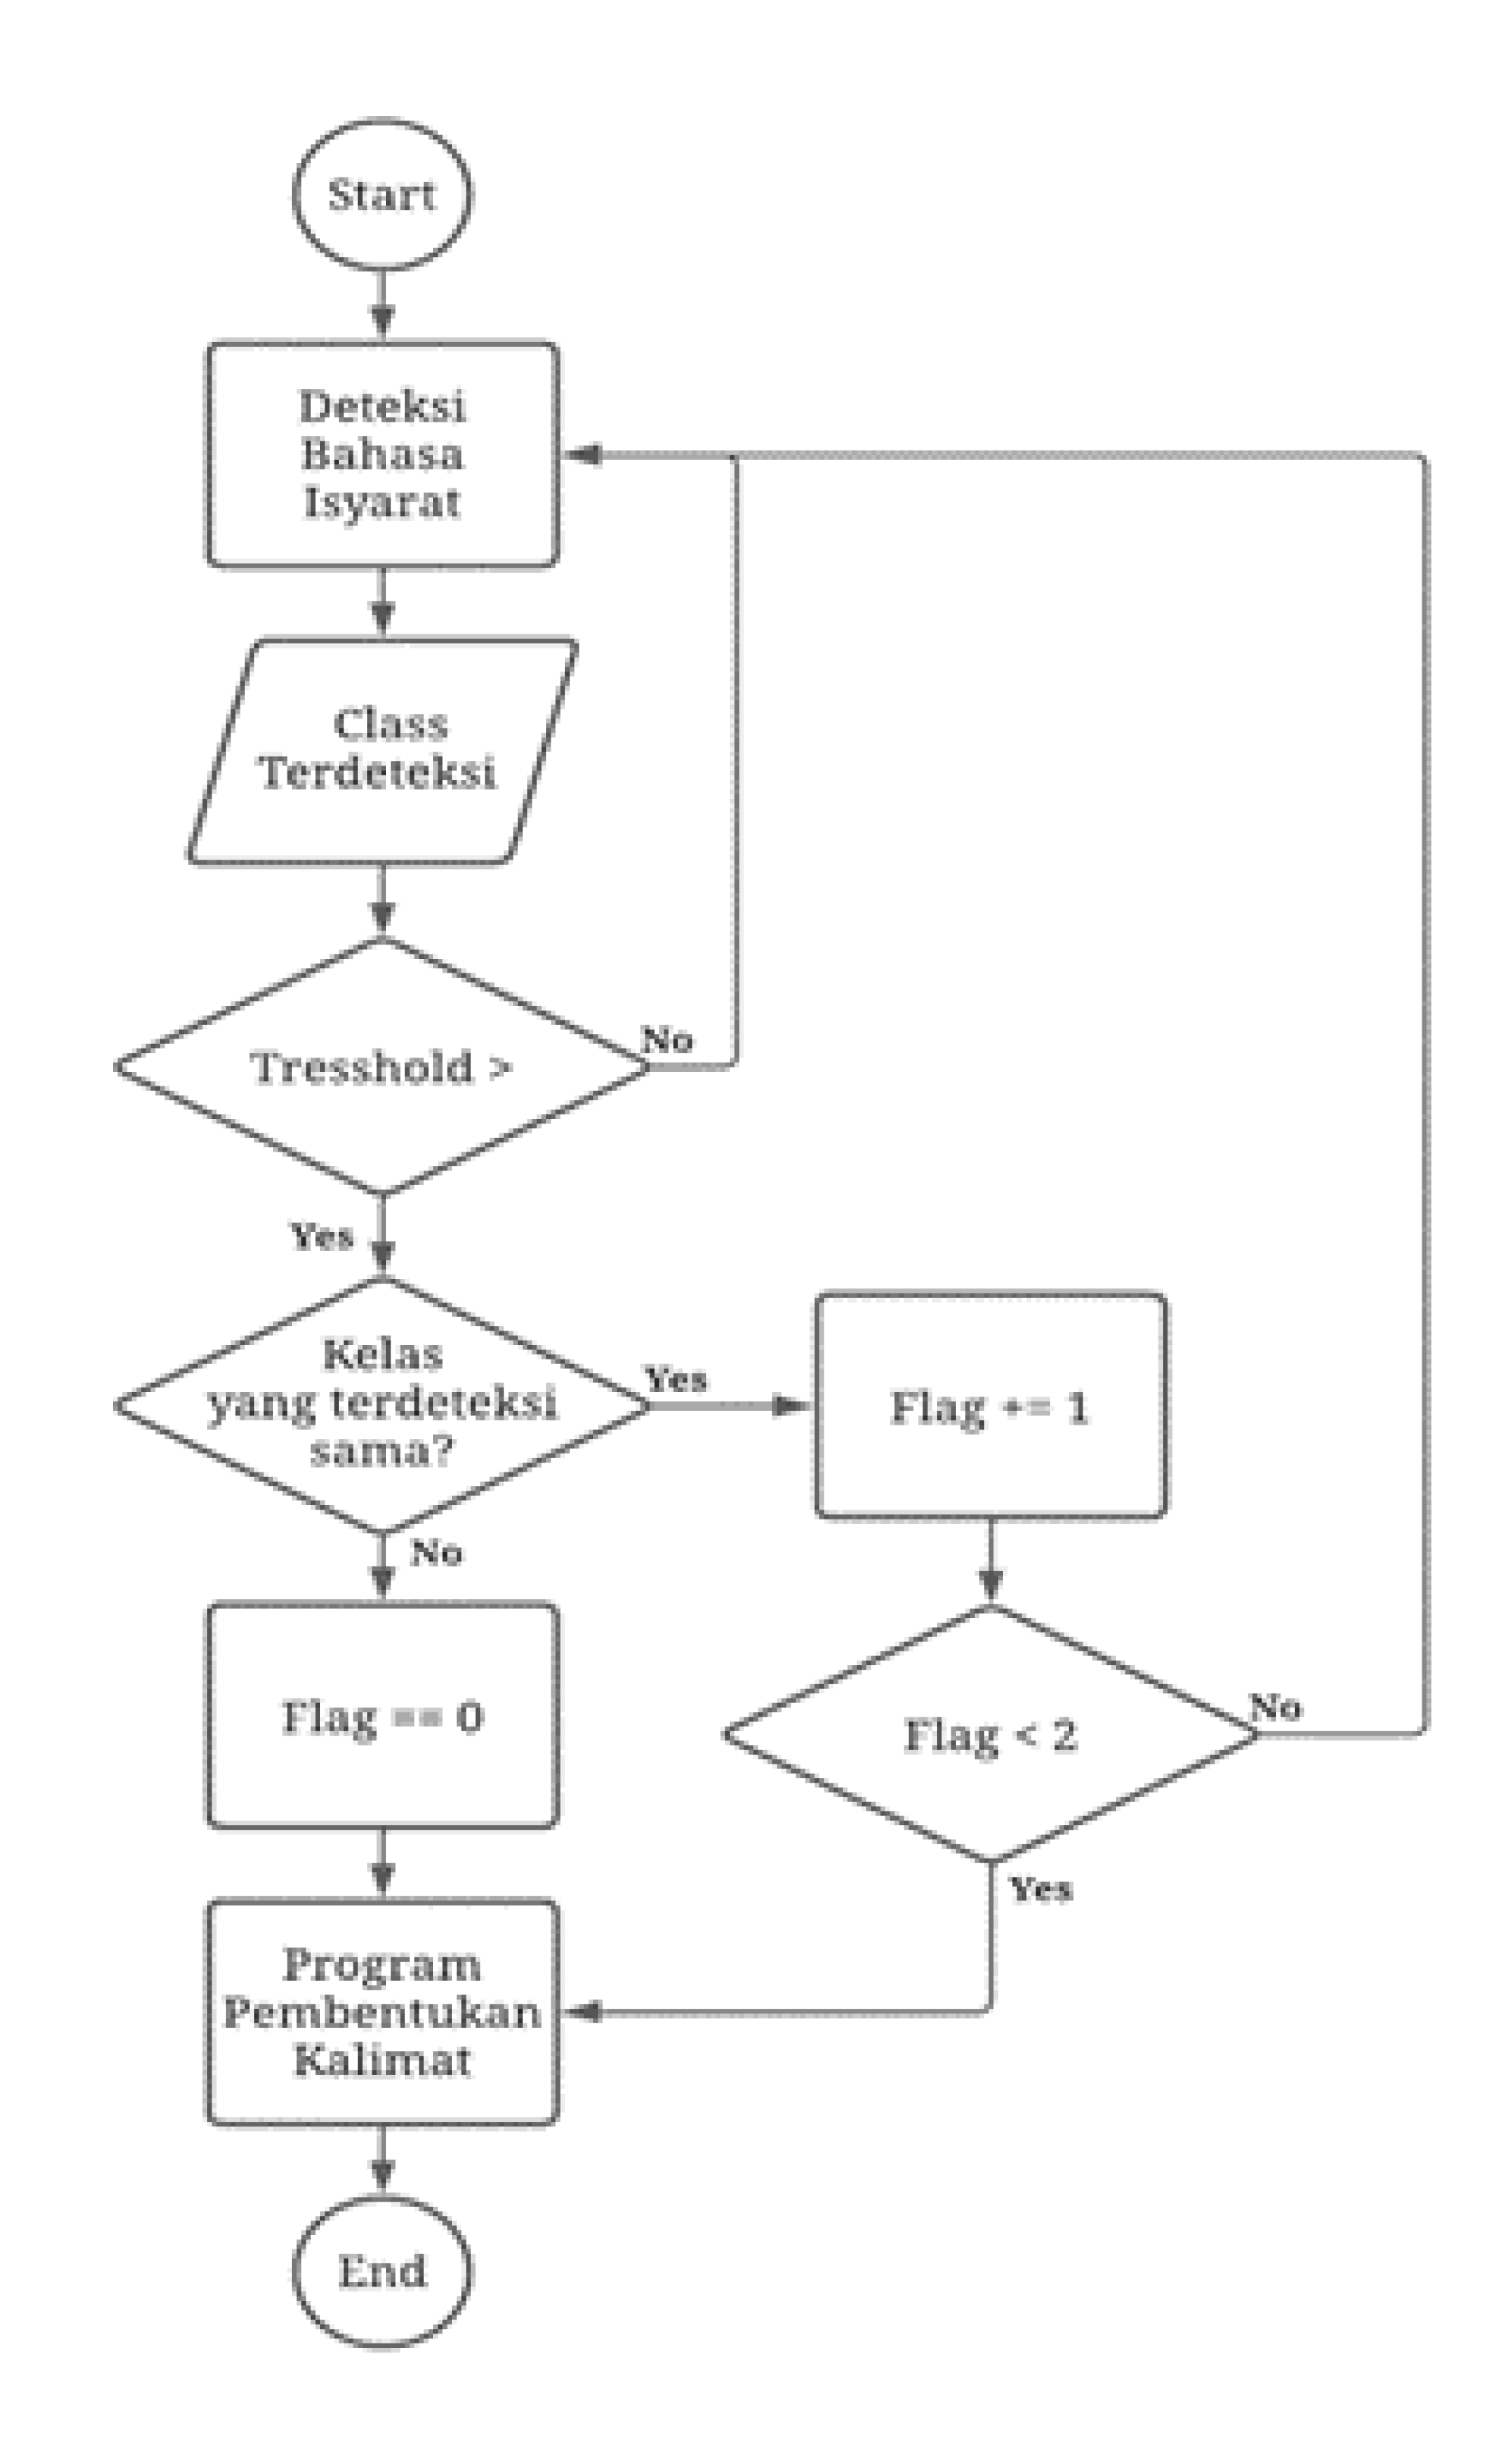
\includegraphics[scale=0.3]{gambar/bab3-flowchart-deteksi.png}

  \caption{Flowchart program deteksi bahasa isyarat}
  \label{fig:flowchartdeteksi}
\end{figure}

\begin{figure}[H]
  \centering

  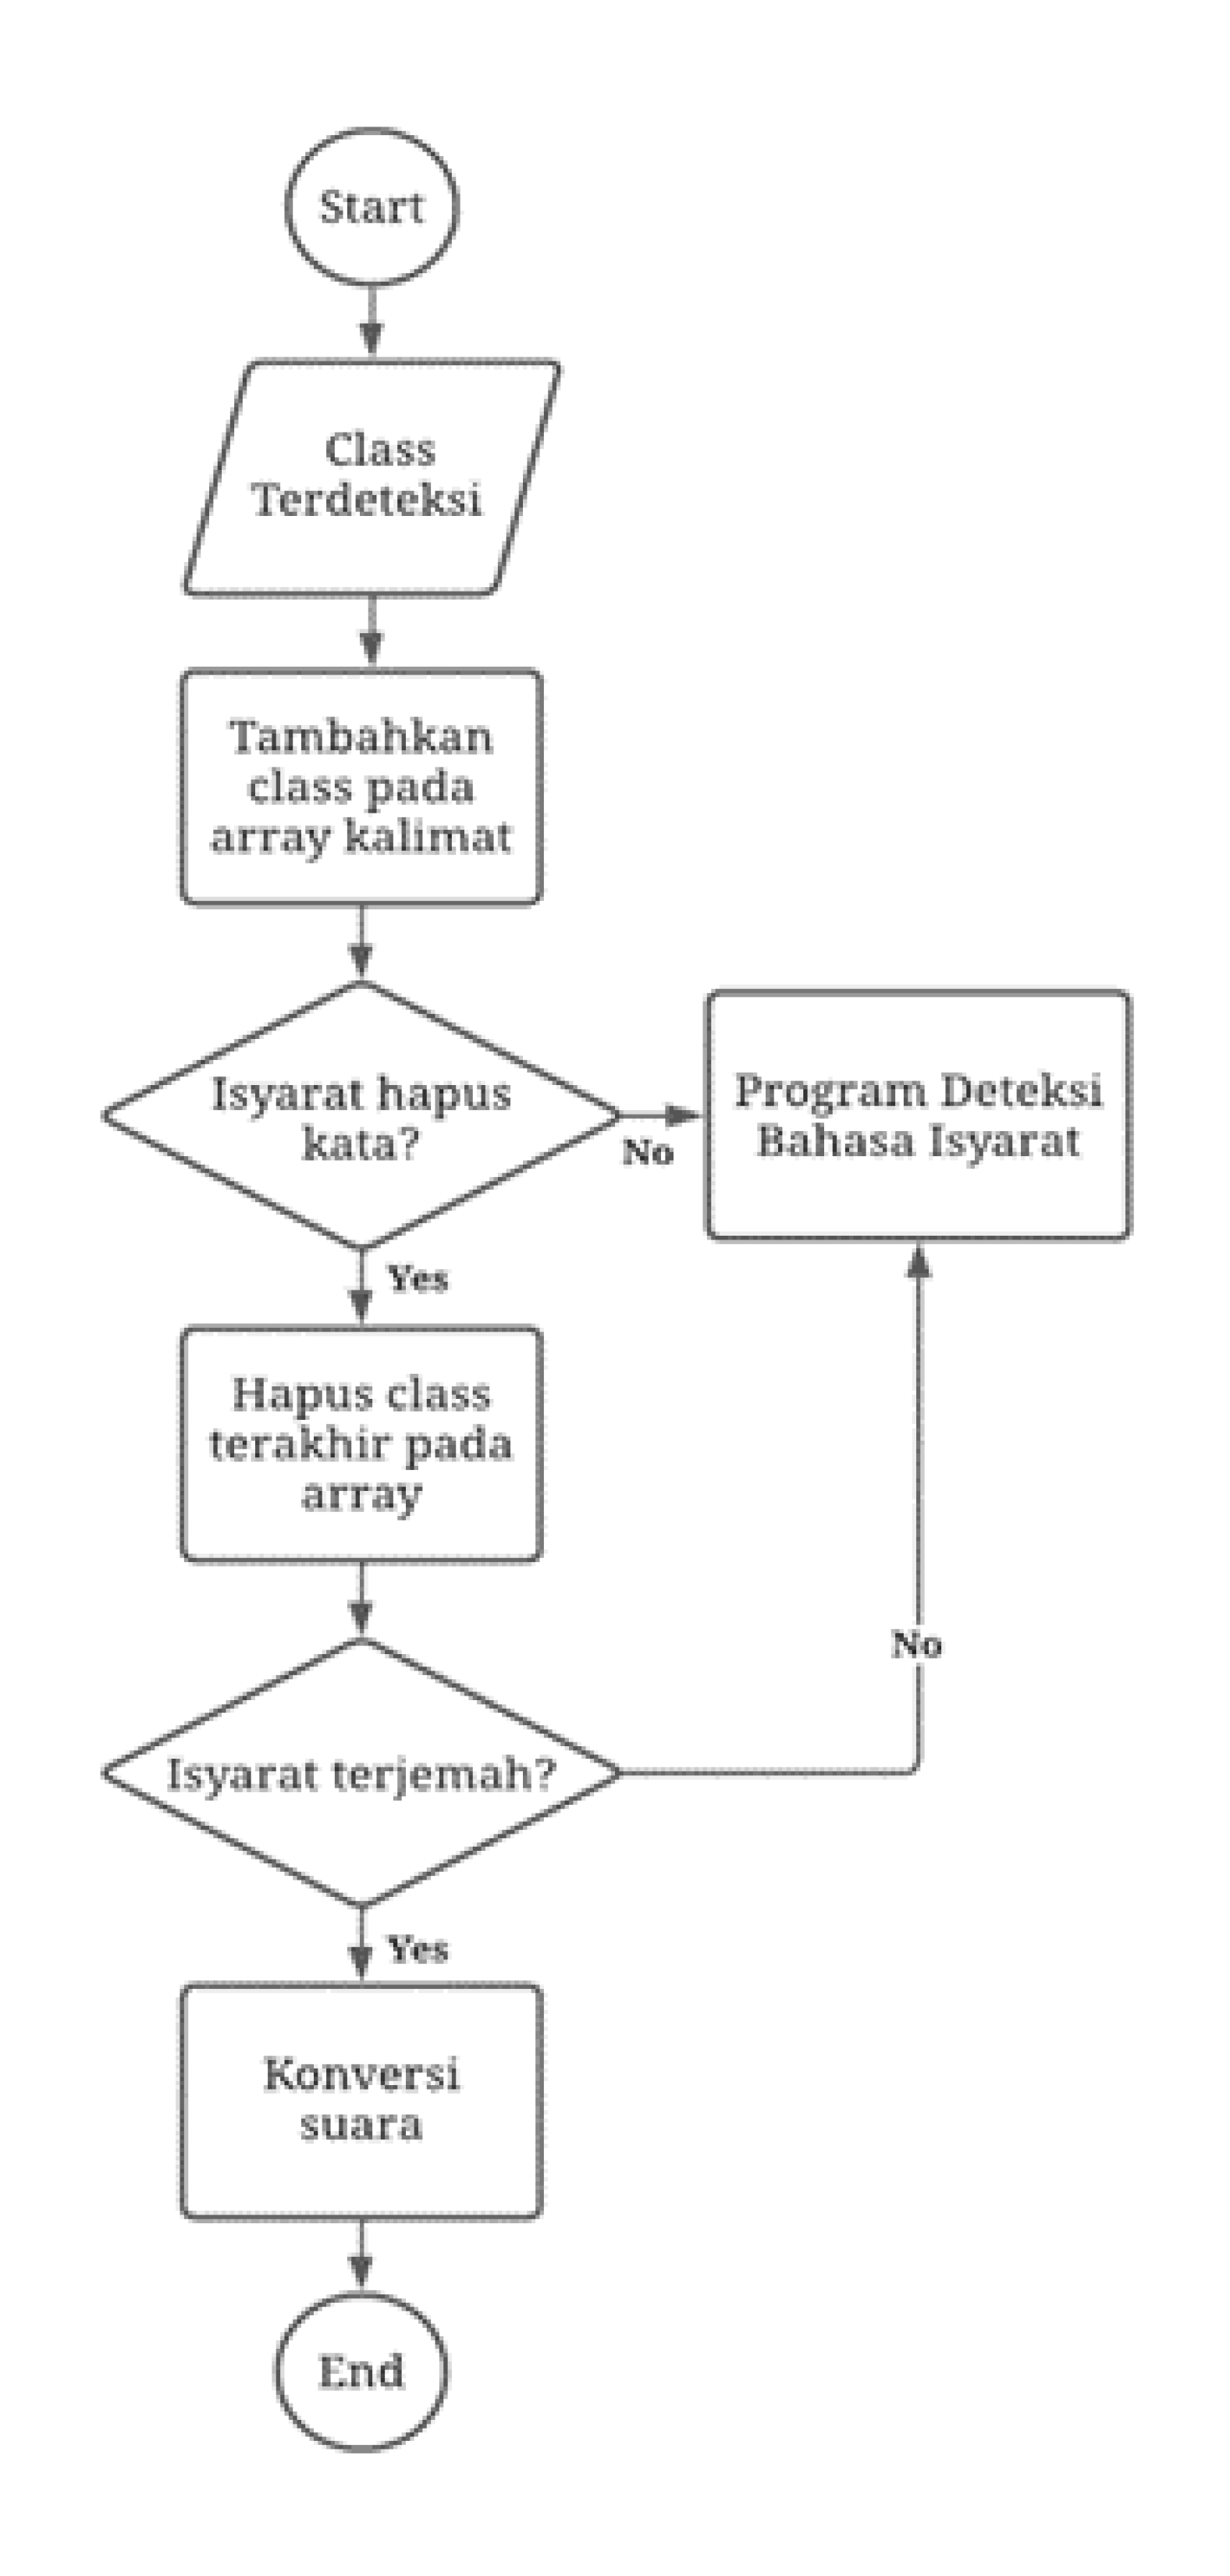
\includegraphics[scale=0.3]{gambar/bab3-flowchart-kalimat.png}

  \caption{Flowchart Program pembentukan kalimat}
  \label{fig:flowchartkalimat}
\end{figure}


\subsection{Integrasi \emph{Next Unit Computing} (NUC)}
\label{subsec:integrasiNUC}

Integrasi dengan Intel NUC dilakukan dengan mengakses website yang dibuat menggunakan \emph{framework} Streamlit penerjemah yang telah terhubung dengan server komputer menggunakan skema \emph{port forwarding}. Website akan mengakses webcam pengguna sehingga pengguna dapat melakukan gerakan isyarat yang kemudian diklasifikasikan dengan model LSTM yang telah dilatih sebelumnya secara \emph{realtime}.

% Pada cetak biru yang tertera pada Gambar \ref{fig:cetakbiru}. \lipsum[8]

% % Contoh input gambar pada kolom.
% \begin{figure} [ht]
%   \centering
%   % Ubah sesuai dengan nama file gambar dan ukuran yang akan digunakan.
%   \includegraphics[width=0.4\textwidth]{gambar/cetakbiru.jpg}

%   % Ubah sesuai dengan keterangan gambar yang diinginkan.
%   \caption{Cetak biru roket yang akan diuji coba. \cite{cetakbiruspacex}}
%   \label{fig:cetakbiru}
% \end{figure}

% \lipsum[9-10]

% \subsection{Lorem Ipsum}
% \label{subsec:loremipsum}

% \lipsum[11]

% % Contoh pembuatan tabel.
% \begin{table}
%   \caption{Contoh tabel sederhana}
%   \label{tab:tabelsederhana}
%   \centering
%   \begin{tabular}{lll}
%     \toprule
%     Heading1 & Heading2 & Heading3 \\
%     \midrule
%     One      & Two      & Three    \\
%     Four     & Five     & Six      \\
%     \bottomrule
%   \end{tabular}
% \end{table}

% % Contoh pembuatan potongan kode.
% \begin{lstlisting}[
%   language=C++,
%   caption={Program halo dunia.},
%   label={lst:halodunia}
% ]
% #include <iostream>

% int main() {
%     std::cout << "Halo Dunia!";
%     return 0;
% }
% \end{lstlisting}

% \lipsum[12]

% % Contoh pembuatan daftar.
% \begin{enumerate}
%   \item \lipsum[13][1-4]
%   \item \lipsum[13][5-8]
%   \item \lipsum[13][9-12]
% \end{enumerate}

% \lipsum[14-15]
% Ubah judul dan label berikut sesuai dengan yang diinginkan.
\section{Hasil dan Pembahasan}
\label{sec:hasildanpembahasan}

% Ubah paragraf-paragraf pada bagian ini sesuai dengan yang diinginkan.

% % Contoh input beberapa gambar pada halaman.
% \begin{figure*}
%     \centering
%     \subfloat[Hasil A]{\includegraphics[width=.4\textwidth]{example-image-a}
%         \label{fig:hasila}}
%     \hfil
%     \subfloat[Hasil B]{\includegraphics[width=.4\textwidth]{example-image-b}
%         \label{fig:hasilb}}
%     \caption{Contoh input beberapa gambar.}
%     \label{fig:hasil}
% \end{figure*}

% \lipsum[16-18]

% % Contoh input potongan kode dari file.
% \lstinputlisting[
%     language=Python,
%     caption={Program perhitungan bilangan prima.},
%     label={lst:bilanganprima}
% ]{program/bilangan-prima.py}

% \lipsum[19-20]

\subsection{Pengujian Bentuk Model}
\label{sec:analisismodel}
Bentuk model yang diujikan dilandaskan oleh bentuk model yang telah dijelaskan pada sub bab \ref{subsec:klasifikasipose}. Pengujian ini dilakukan untuk mengamati bagaimana pengaruh struktur model LSTM terhadap performa klasifikasi dari gerakan bahasa isyarat. Adapun perbedaan pada layer yang digunakan adalah sebagai berikut:

\begin{table}[H]
    \caption{Struktur Model LSTM}
    \label{tb:ringkasanModel}
    \centering
    \begin{tabular}{ll}
      \hline
      \textbf{Model} & \textbf{Struktur Layer} \\
      \hline
      Model 1 & 
      \begin{tabular}[t]{l}
        \emph{LSTM} 1 (128 unit, \emph{relu}) \\
        \emph{Dropout} 1 (0.5) \\
        \emph{LSTM} 2 (64 unit, \emph{relu}) \\
        \emph{Dropout} 2 (0.5) \\
      \end{tabular} \\
      \hline
      Model 2 & 
      \begin{tabular}[t]{l}
        \emph{TimeDistributed} (\emph{Dense}, 128 unit, \emph{tanh}) \\
        \emph{LSTM} 1 (64 unit, \emph{tanh}) \\
        \emph{Dropout} 1 (0.5) \\
      \end{tabular} \\
      \hline
      Model 3 & 
      \begin{tabular}[t]{l}
        \emph{TimeDistributed} (\emph{Dense}, 128 unit, \emph{tanh}) \\
        \emph{LSTM} 1 (128 unit, \emph{tanh}) \\
        \emph{Dropout} 1 (0.5) \\
        \emph{LSTM} 2 (64 unit, \emph{tanh}) \\
        \emph{Dropout} 2 (0.5) \\
      \end{tabular} \\
      \hline
    \end{tabular}
  \end{table}
  
Model dilatih dengan \emph{epoch} sebanyak 12 dengan partisi dataset sebesar 70:30, 70\% data training dan 30\% data validasi. Model yang telah dilatih kemudian diuji berdasarkan data testing yang ada dan memberikan hasil klasifikasi sebagai berikut:

\begin{table}[H]
    \caption{Hasil Evaluasi Model LSTM}
    \label{tb:evaluasiModel}
    \centering
    \begin{tabular}{lllll}
      \hline
      \textbf{Model} & \textbf{\emph{Avg. Accuracy}} & \textbf{\emph{Avg. Precision}} & \textbf{\emph{Avg. Recall}} & \textbf{\emph{Avg. F1-Score}} \\
      \hline
      Model 1 & 0.85 & 0.85 & 0.85 & 0.83 \\
      Model 2 & 0.93 & 0.95 & 0.94 & 0.94 \\
      Model 3 & 0.99 & 0.99 & 0.98 & 0.99 \\
      \hline
    \end{tabular}
  \end{table}
  
Berdasarkan tabel \ref{tb:evaluasiModel} dapat dilihat bahwa adanya relasi antara peningkatan kompleksitas dari model LSTM mempengaruhi performa klasifikasi gerakan bahasa isyarat. Hal ini dapat dilihat bahwa pada model ketiga menghasilkan performa terbaik dengan penggunaan \emph{layer} TimeDistributed dan 2 \emph{layer} LSTM.

\subsection{Pengujian Kondisi Cahaya}
\label{sec:analisiscahaya}

Pengujian ini akan dilihat bagaimana kemampuan adaptasi model terhadap perubahan intensitas cahaya dari ruangan. Pengujian ini dilakukan dengan menggunakan model ketiga yang telah diujikan pada tabel \ref{tb:ringkasanModel} dengan jarak pengguna 300 cm dari kamera. Pengambilan data intensitas cahaya dilakukan dengan aplikasi Lux Meter.

\begin{table}[H]
  \caption{Hasil Evaluasi Tingkat Cahaya}
  \label{tb:evaluasiCahaya}
  \centering
  \begin{tabular}{llll}
    \hline
    \textbf{Cahaya} & \textbf{Akurasi} & \emph{\textbf{Avg. Processing Time}} & \emph{\textbf{Avg. Complete Time}} \\
    \hline
    35 lux & 0.89 & 0.0938 & 3.0335 \\
    80 lux & 1.00 & 0.0918 & 2.9928 \\
    125 lux & 0.96 & 0.0923 & 2.4777 \\
    \hline
  \end{tabular}
\end{table}

Berdasarkan tabel \ref{tb:evaluasiCahaya} dapat dilihat bahwa adanya penurunan intensitas cahaya pada suatu ruangan menyebabkan adanya peningkatan pada \emph{processing time} dan \emph{complete time}. Namun apabila dilihat pada aspek akurasi, dapat dilihat bahwa intensitas cahaya 125 lux memiliki akurasi terbaik jika dibandingkan dengan intensitas cahaya lainnya. Hal ini disebabkan oleh peningkatan intensitas cahaya menyebabkan kamera dapat menangkap gerakan isyarat dengan lebih jelas.


\subsection{Pengujian Kondisi Jarak}
\label{sec:analisisjarak}

Pengujian ini akan dilihat bagaimana kemampuan adaptasi model terhadap perubahan jarak pengguna terhadap kamera.  Pengujian ini dilakukan dengan menggunakan model ketiga yang telah diujikan pada tabel \ref{tb:ringkasanModel} dengan intensitas cahaya bernilai 125 lux. Perlu diperhatikan bahwa gerakan isyarat pengguna dapat harus terlihat secara jelas pada kamera. 

\begin{table}[H]
  \caption{Hasil Evaluasi Jarak}
  \label{tb:evaluasiJarak}
  \centering
  \begin{tabular}{llll}
    \hline
    \textbf{Jarak} & \textbf{Akurasi} & \emph{\textbf{Avg. Processing Time}} & \emph{\textbf{Avg. Complete Time}} \\
    \hline
    180 cm & 0.89 & 0.1017 & 2.3660 \\
    240 cm & 0.96 & 0.0994 & 2.5098 \\
    300 cm & 1.00 & 0.0997 & 2.7918 \\
    \hline
  \end{tabular}
\end{table}

Berdasarkan tabel \ref{tb:evaluasiJarak} dapat dilihat bahwa peningkatan jarak menghasilkan klasifikassi model dengan akurasi yang lebih baik. Hal ini disebabkan oleh kemudahan kamera menangkap dengan jelas gerakan isyarat yang dilakukan oleh pengguna seiring dengan peningkatan jarak. Namun, peningkatan jarak mengakibatkan peningkatan pada \emph{complete time}. Pada \emph{processing time} cenderung bernilai fluktuatif.

\subsection{Pengujian Subjek Berbeda}
\label{sec:analisissubjek}

Pengujian ini dilakukan untuk melihat kemampuan adaptasi model terhadap perubahan subjek selain pengguna. Pengujian ini dilakukan dengan menggunakan model ketiga yang telah diujikan pada tabel \ref{tb:evaluasiModel} dengan intensitas cahaya bernilai 125 lux dan jarak terhadap kamera bernilai 300 cm. Subjek yang mengikuti pengujian ini dapat dlihat pada tabel \ref{tb:kondisisubjek}

\begin{table}[H]
  \caption{Variasi Subjek Berbeda}
  \label{tb:kondisisubjek}
  \centering
  \begin{tabular}{ll}
    \hline
    \textbf{Jenis Kelamin} & \textbf{Gambar Subjek} \\
    \hline
    Perempuan & 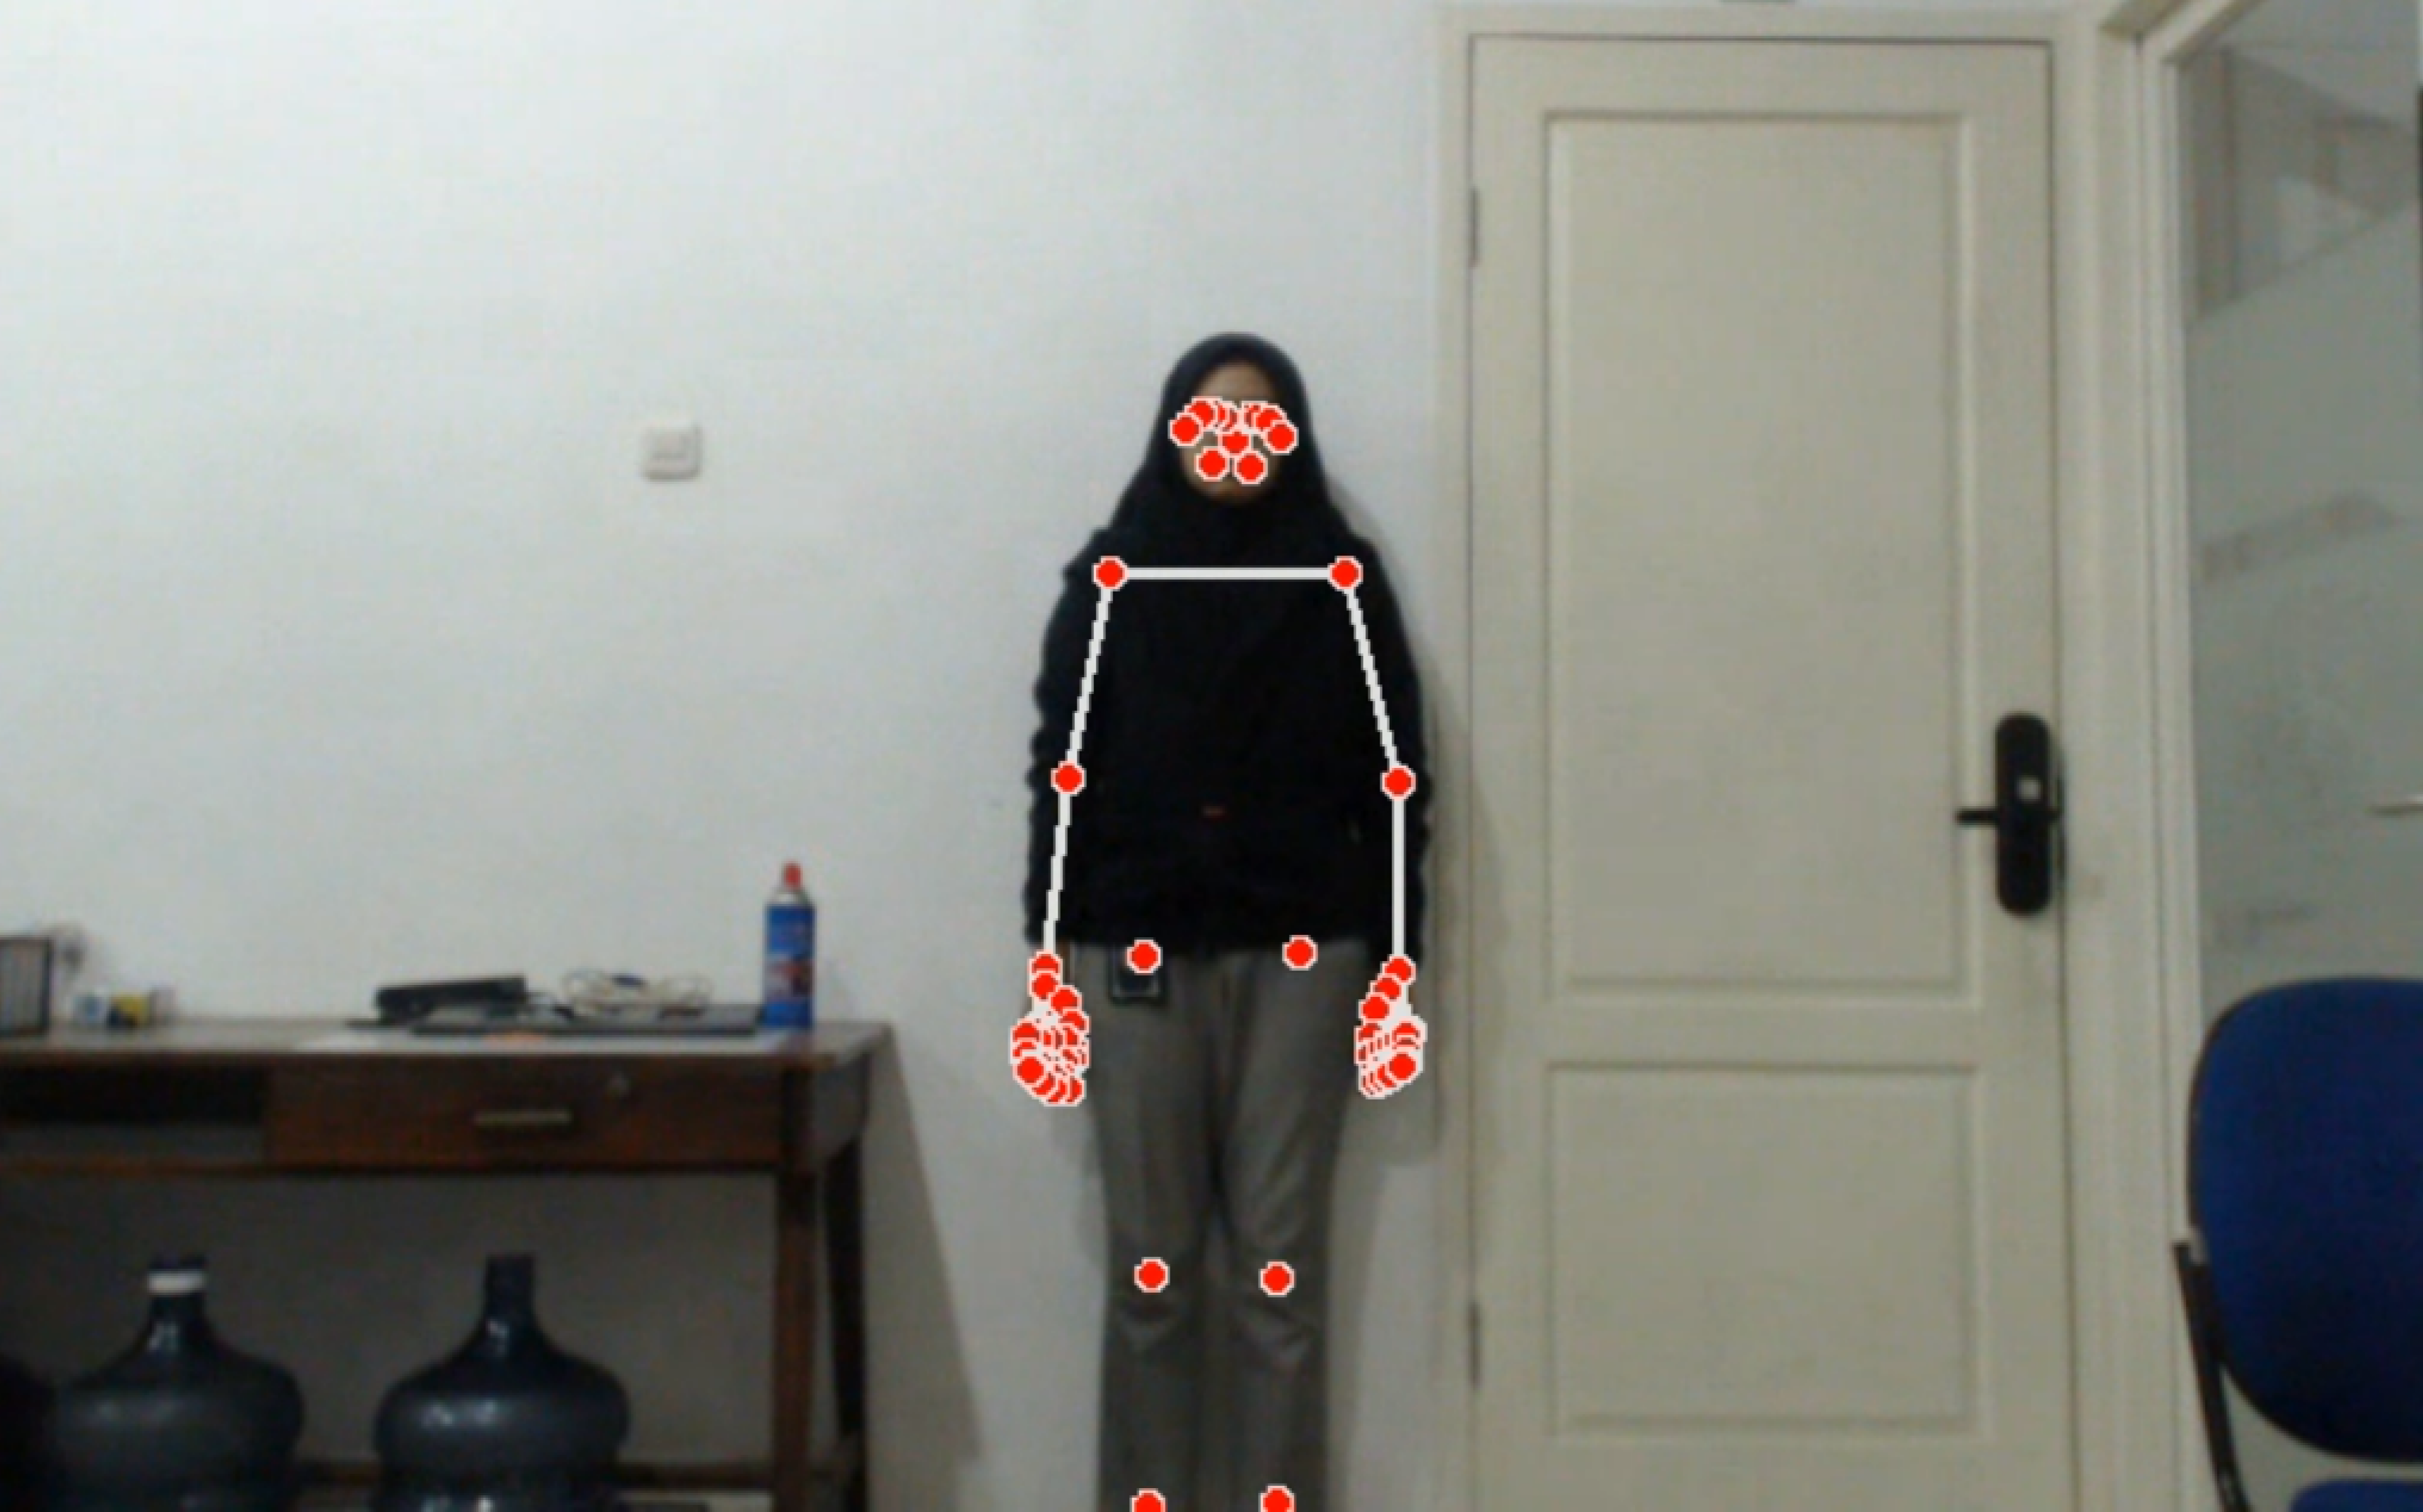
\includegraphics[scale=0.12]{gambar/bab4-rani.png} \\
    \hline
    Laki - Laki & 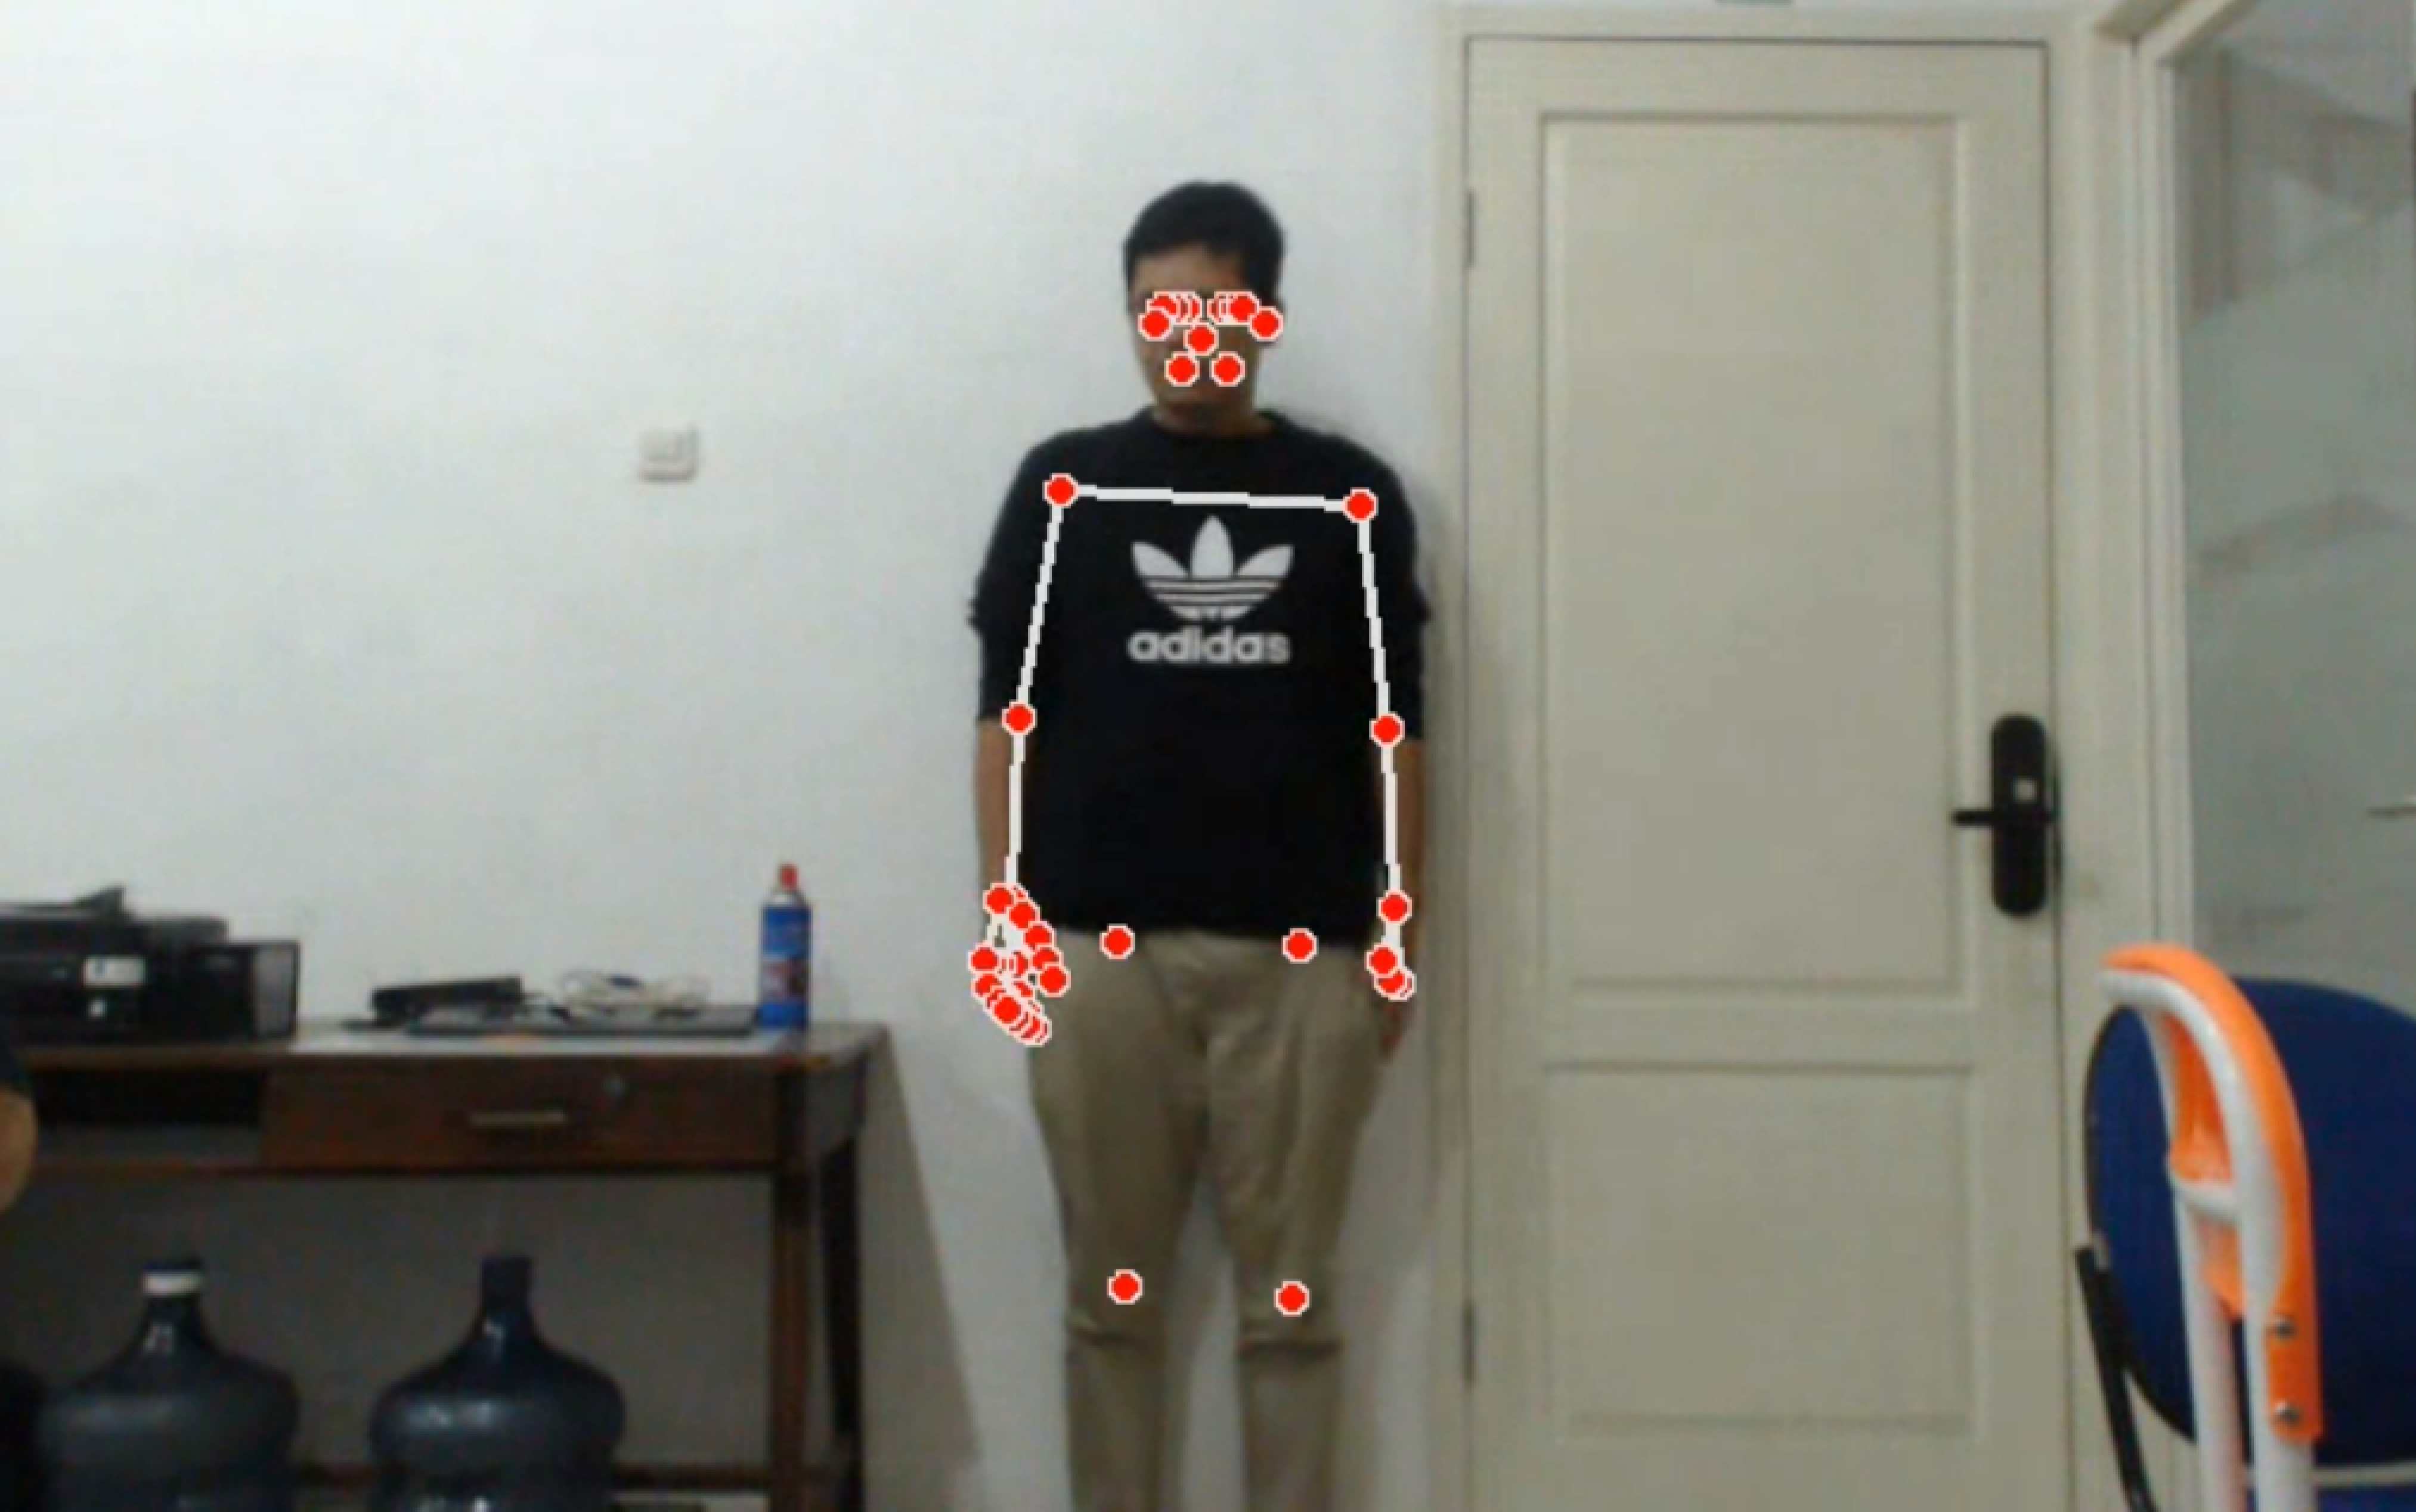
\includegraphics[scale=0.12]{gambar/bab4-evan.png} \\
    \hline
  \end{tabular}
\end{table}

\begin{table}[H]
  \caption{Hasil Evaluasi Subjek Berbeda}
  \label{tb:evaluasiSubjek}
  \centering
  \begin{tabular}{llll}
    \hline
    \textbf{Subjek} & \textbf{Accuracy} & \emph{\textbf{Avg. Processing Time}} & \emph{\textbf{Avg. Complete Time}} \\
    \hline
    Perempuan & 0.93 & 0.0988 & 2.6636 \\
    Laki - Laki & 0.93 & 0.0973 & 2.8191 \\
    \hline
  \end{tabular}
\end{table}

Berdasarkan tabel \ref{tb:evaluasiSubjek} dapat dilihat bahwa model dapat melakukan klasifikasi pada subjek yang berbeda. Normalisasi data telah menghasilkan model yang \emph{scale invariant} dan \emph{position invariant}. Adapun akurasi klasifikasi model menunjukkan nilai yang sangat baik, yaitu bernilai 0.93 atau 93\%. \emph{Average processing time} dan \emph{complete time} juga menunjukkan nilai yang tidak jauh dengan pengujian yang dilakukan oleh penulis sebelumnya, yaitu untuk \emph{average processing time} berkisar pada 0.098 dan untuk \emph{complete time} berkisar pada 2.74. 

\subsection{Pengujian Pembentukan Kalimat dan Konversi Suara}
\label{sec:analisiskalimat}

Pengujian ini dilakukan untuk memahami bagaimana sistem penerjemah digunakan untuk membentuk serangkaian kalimat dan melakukan konversi suara berdasarkan kalimat yang dibentuk. Dalam membentuk kalimat pada sistem ini merujuk pada sub bab \ref{subsec:sisitemkontrol}. Kalimat akan dibentuk berdasarkan kombinasi dari kosakata yang terdeteksi. Kombinasi kosakata secara lengkap pada tabel \ref{tb:kombinasiKosakata}. Pengujian ini dilakukan dengan menggunakan model ketiga yang telah diujikan pada tabel \ref{tb:evaluasiModel} dengan intensitas cahaya bernilai 125 lux dan jarak terhadap kamera bernilai 300 cm. Maksimal perulangan yang dilakukan adalah sebanyak 3 kali untuk masing - masing kosakata. Untuk setiap kombinasi kosakata juga dilakukan pengujian terhadap kosakata kontrol, meliputi "standby", "\emph{delete}", dan "\emph{translate}".

\begin{table}[H]
  \caption{Kombinasi Kosakata dan Kalimat}
  \label{tb:kombinasiKosakata}
  \centering
  \begin{tabular}{ll}
    \hline
    \textbf{Kombinasi Kosakata} & \textbf{Kalimat} \\
    \hline
    "Maaf" + "Siapa" + "Nama" & "Maaf siapa nama kamu?" \\
    "Maaf" + "Tolong" + "Saya" & "Maaf tolong bantu saya" \\
    "Maaf" + "Rumah" + "Siapa" & "Maaf ini rumah siapa?" \\
    "Rumah" + "Saya" & "Ini rumah saya" \\
    "Rumah" + "Siapa" & "Ini rumah siapa?" \\
    "Siapa" + "Nama" & "Siapa nama kamu?" \\
    "Tolong" + "Saya" & "Tolong bantu saya" \\
    \hline
  \end{tabular}
\end{table}


\begin{table}[H]
  \caption{Hasil Evaluasi Kombinasi Kosakata}
  \label{tb:evaluasiKombinasi}
  \centering
  \begin{tabular}{llll}
    \hline
    \textbf{Kombinasi} & \textbf{Akurasi} & \emph{\textbf{Avg. Processing Time}} & \emph{\textbf{Avg. Complete Time}} \\
    \hline
    2 kosakata & 1.00 & 0.0993 & 2.8303 \\
    3 kosakata & 0.93 & 0.0981 & 2.0513 \\
    \hline
  \end{tabular}
\end{table}

Dapat dilihat pada tabel \ref{tb:evaluasiKombinasi} bahwa model telah berhasil membentuk kalimat dengan melakukan kombinasi secara sekuensial dan berkelanjutan. Hal ini ditunjukkan dengan akurasi pada kalimat yang dibentuk dari kombinasi 2 kosakata bernilai 1.00 dan kombinasi 3 kosakata bernilai 0.93. Untuk nilai \emph{average processing time} dan nilai \emph{average complete time} tidak mengalami perubahan yang signifikan dengan pengujian yang berjalan secara berkelanjutan. Adapun dalam pembentukan kalimat "Ini rumah saya", terdapat kesalahan dalam klasifikasi gerakan isyarat "rumah" yang diklasifikasikan sebagai "delete". Hal ini disebabkan oleh tingkat kemiripan yang cukup tinggi antara gerakan isyarat "rumah" dan "delete". Secara keseluruhan, tingkat keberhasilan sistem dalam membentuk kalimat adalah 0.857 atau 85.7\%.

Berdasarkan keseluruhan pengujian yang dilakukan menunjukkan bahwa sistem memiliki performa yang baik dalam penerjemahan gerakan isyarat dalam jumlah yang relatif banyak dan secara \emph{realtime}.

\begin{figure}[ht]
    \centering

    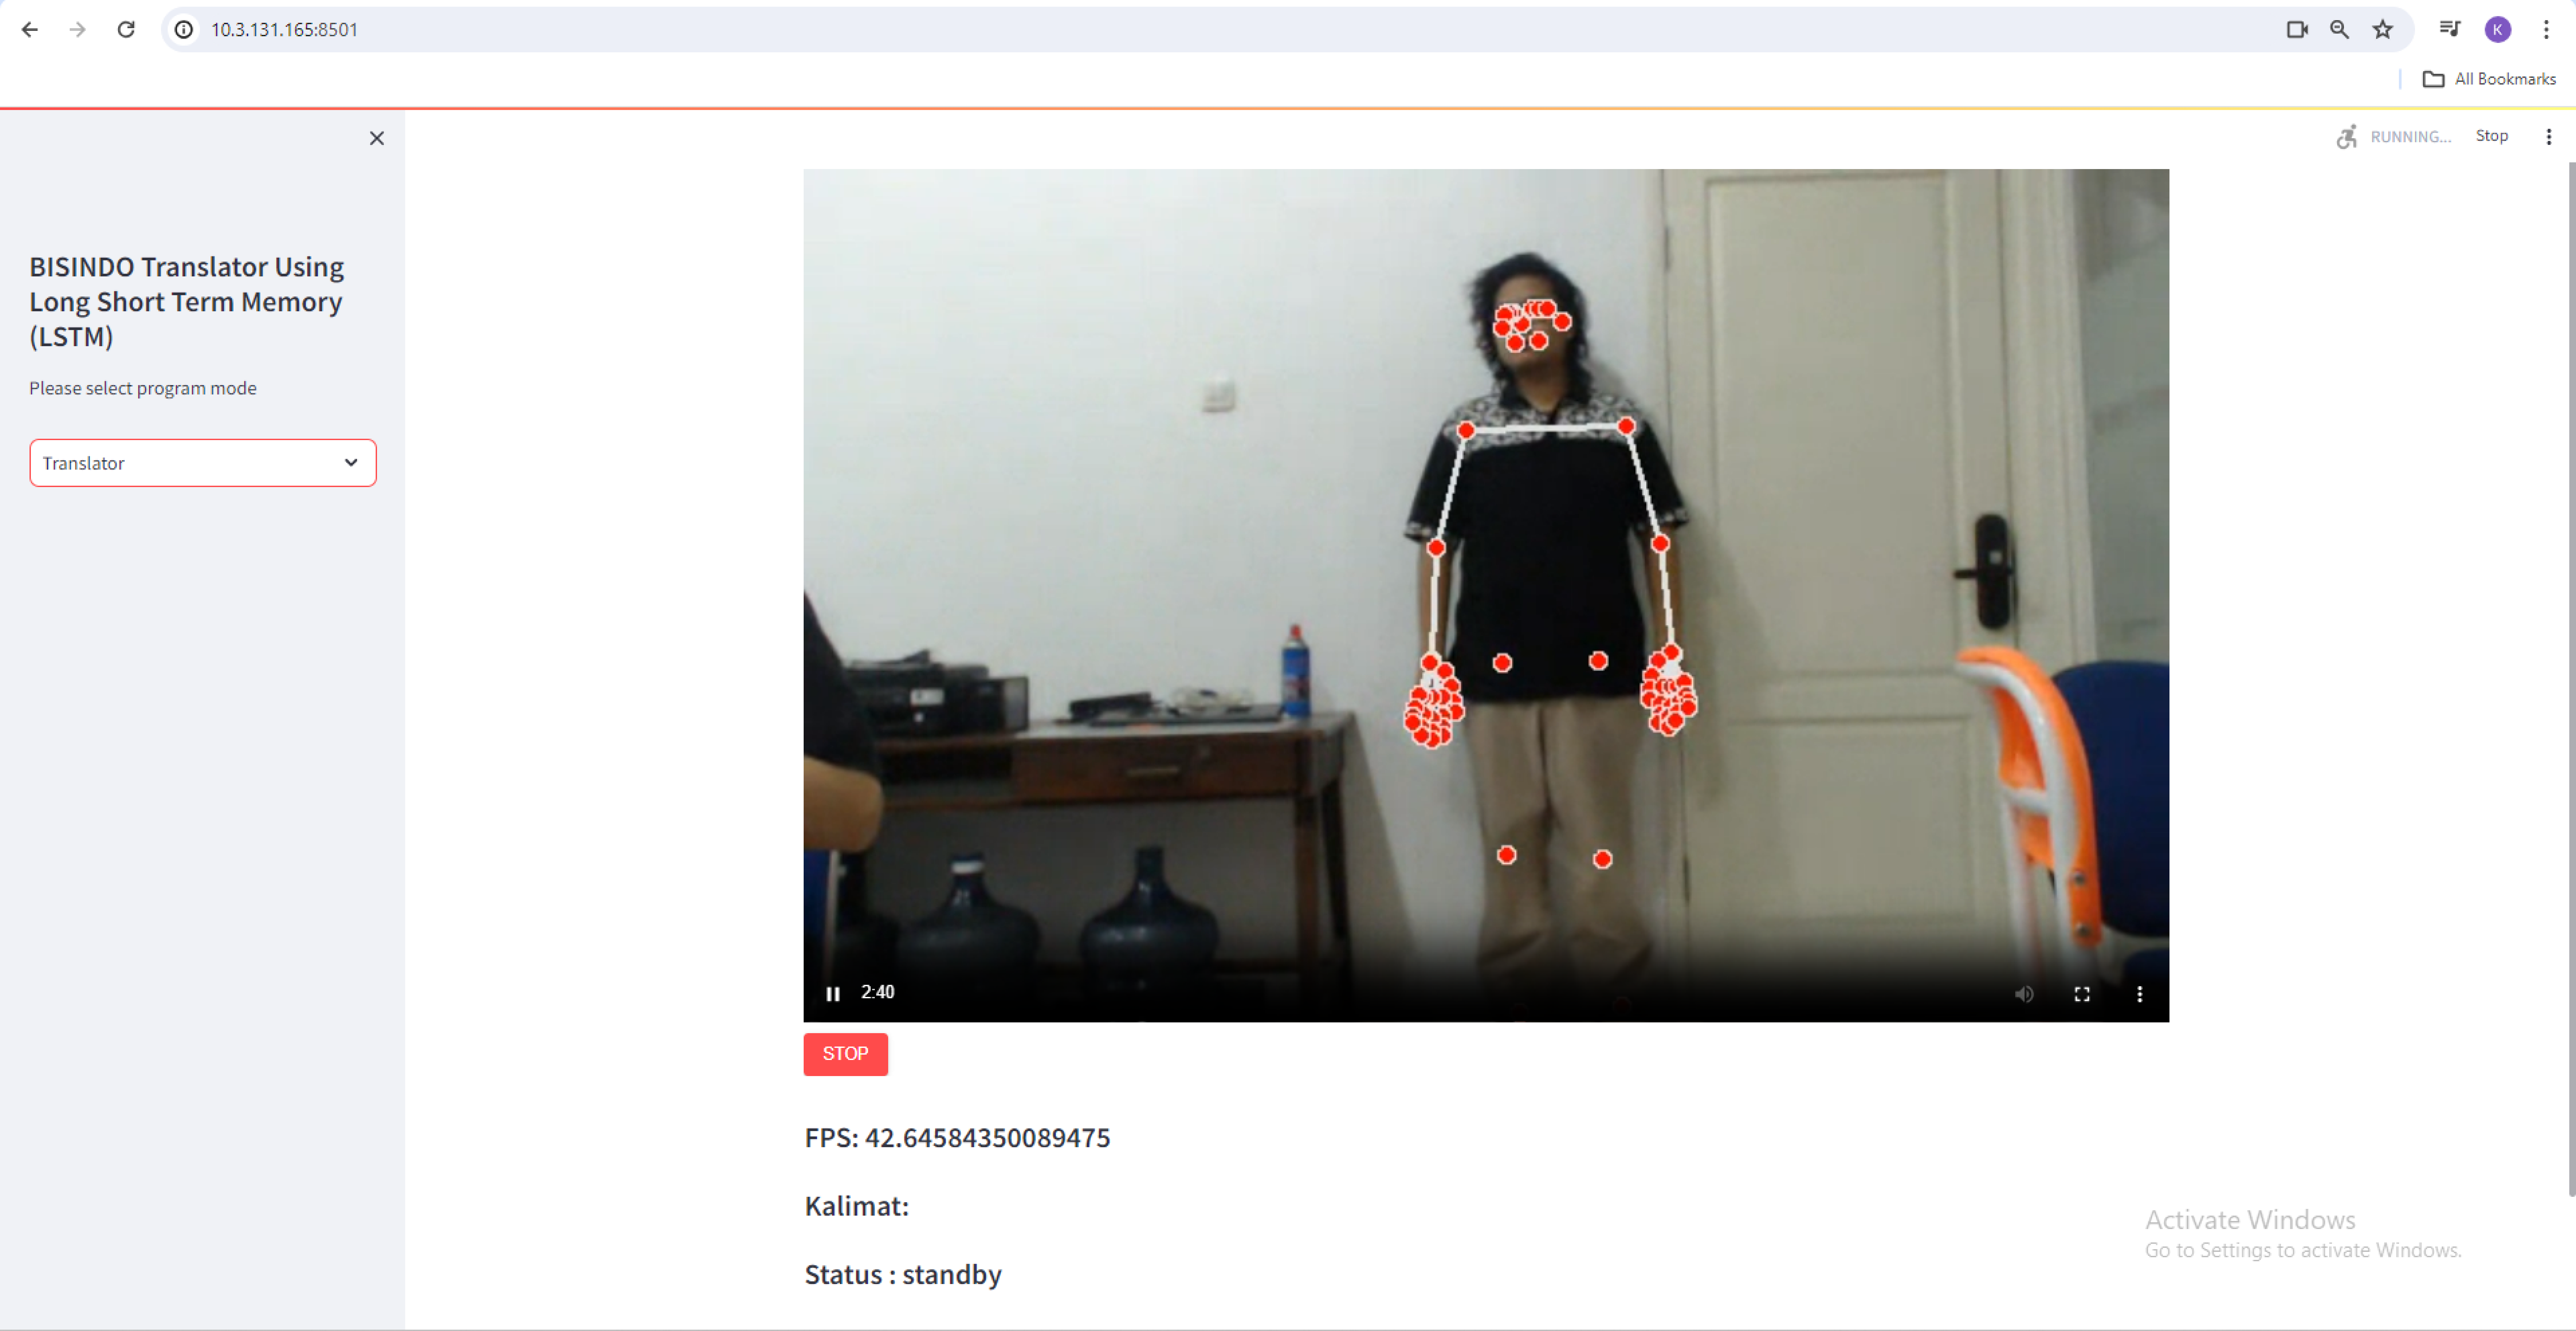
\includegraphics[scale=0.12]{gambar/bab3-layoutweb.png}
 
    \caption{Hasil Pengujian Sistem}
    \label{fig:layoutweb}
\end{figure}
% Ubah judul dan label berikut sesuai dengan yang diinginkan.
\section{Kesimpulan}
\label{sec:kesimpulan}

% Ubah paragraf-paragraf pada bagian ini sesuai dengan yang diinginkan.

Berdasarkan penelitian yang telah dilaksanakan dapat diambil kesimpulan sebagai berikut:

\begin{enumerate}[nolistsep]
      \item Sistem penerjemah bahasa isyarat telah berhasil diimplementasikan pada Intel \emph{Next Unit Computing} (NUC) dan dapat berjalan secara \emph{real time}. 
  \item Model LSTM memiliki performa paling baik dengan penggunaan \emph{layer TimeDistributed} yang diikuti dengan 2 \emph{layer} LSTM pada akurasi 99\%.
  \item Intensitas cahaya 125 lux atau kondisi ruangan terang menghasilkan klasifikasi terbaik dengan akurasi sebesar 100\% dan dengan nilai rata - rata FPS yang relatif tinggi, yaitu 12.905.
  \item Jarak kamera terhadap pengguna sebesar 300 cm menghasilkan klasifikasi terbaik dengan akurasi sebesar sebesar 100\%, namun dengan nilai rata - rata FPS yang relatif rendah, yaitu 10.746.
  \item Model berhasil beradaptasi dengan subjek selain penulis dengan akurasi sebesar 92.5\% untuk subjek perempuan dan laki - laki dengan nilai rata - rata FPS yang relatif tinggi, yaitu bernilai 11.702.
  \item Sistem penerjemah dapat membentuk kalimat dan mengkonversi menjadi suara dengan tingkat keberhasilan sebesar 85.7 dengan rata - rata nilai FPS yang relatif tinggi, yaitu 11.678\%.
  
\end{enumerate}

Berdasarkan penelitian yang telah dilakukan, adapun saran yang dapat dipertimbangkan untuk pengembangan lebih lanjut adalah sebagai berikut:

\begin{enumerate}[nolistsep]

  \item Menambahkan variasi jarak, intensitas cahaya, dan subjek berbeda untuk menguji bagaim\\ana kemampuan model dalam beradaptasi dengan serangkaian perubahan yang terjadi.
  \item Mempertimbangkan menggunakan metode lain, seperti CNN-LSTM untuk dapat melakukan ekstraksi \emph{feature} dalam bentuk citra sehingga dapat melakukan klasifikasi gerakan bahasa isyarat dengan lebih baik dan akurat lagi.

\end{enumerate}
% Ucapan terima kasih jika ada
\input{konten/id/6-ucapan-terima-kasih.tex}

% Menampilkan daftar pustaka dengan format IEEE
\bibliographystyle{IEEEtranN}
\bibliography{pustaka/pustaka.bib}

% Menyeimbangkan bagian akhir di kedua kolom
\balance

\end{document}
